\documentclass[midd]{thesis}

\usepackage{graphicx}
\usepackage{times}
\usepackage{listings}
\usepackage{changepage}
\usepackage{longtable}
\lstset{
    basicstyle=\linespread{1}\ttfamily,
}

\bibliographystyle{plain}

\title {Examining the Security of Local Inter-Process Communication}

\author {Brendan Leech}
\adviser {Professor Peter C. Johnson}

\begin{document}

\maketitle
\pagenumbering{roman}

\begin{abstract}
Local inter-process communication allows processes on the same computer to share data.  Even though this communication stays within a single computer, best practices for computer security must still be followed.  In this thesis, I investigate the security of local inter-process communication for four different applications.  While I did not find bugs in the vast majority of local IPC endpoints that I studied, I did find one bug due to incorrect input parsing and validating invalid input.  Additionally, I created two Denial-of-Service attacks that prevent a user from opening an application and interacting with much of the Internet.  These three findings underscore the lack of emphasis given to local IPC security and highlight the need to focus more on this in the future.
\end{abstract}

\begin{acknowledgements}
I'd like to thank my advisor, Pete, for all of his help this semester and throughout the six other classes I have been lucky enought to take with him.  This project would not have been a success without his advice and guidance throughout the past four years and particularly throughout this thesis process.  I also could not have made it this far in my computer science education without the other amazing professors I have had here at Middlebury College, especially Professor Briggs and Professor Christman, each of whom I took multiple classes with throughout my time in the Middlebury CS department.  I'd also like to thank the people who took my survey, which helped inform my decision of what applications to investigate.  Finally, I want to thank my friends and family who supported me throughout the semester, especially those who helped run some of my tests as time was running out.
\end{acknowledgements}

\contentspage
\tablelistpage   % comment this out if you don't have any tables
\figurelistpage

\normalspacing \setcounter{page}{1} \pagenumbering{arabic}

\chapter{Introduction}
\label{sec:intro}

Many modern applications split functionality into multiple processes, allowing programmers to achieve the design principle of separation of concerns.  For example, by creating a password manager that uses two processes, one to store the passwords and a second to display them to the user, programmers can separately focus on the two very different tasks.  One group can ensure that the stored passwords are unable to be stolen from the machine, while the other can provide the interface between the user and his or her information.  This division of labor also allows someone with security expertise to only work on keeping the passwords safe and a user-interface designer to create a functional UI, instead of having one group work in areas that are not their strengths.  However, separating related operations into different processes implies that they must communicate in some way.  The password manager needs some way of getting the passwords from the secured database to the UI for the user to view.  This is an example of inter-process communication.

\section{Inter-Process Communication}
\label{sec:ipcIntro}
Inter-process communication encompasses any form of communication between running processes.  This is a very broad definition that applies to much of the way that people use computers.  Inter-process communication, or IPC, captures everything from email to using a web browser to get webpages from a web server to password managers transmitting passwords within a computer.  Local IPC is communication that occurs within a single computer.  Instead of traversing the Internet and interacting with many hosts, local inter-process communication stays completely inside one computer, and is often dealt with entirely by the kernel.  Inter-process communication and local IPC will be further explored in Chapter~\ref{sec:interProcessCommunication}.

\section{Insecurity of Inter-Process Communication}
\label{sec:ipcInsecurity}
\subsection{What does it mean to be insecure?}
\label{sec:whatIsInsecure}
For an application to be insecure, an attacker must be able to exploit the application to act in a way that is not desired.  These attacks can be broken down into two broad classes: information disclosure and execution hijacking.  An information disclosure attack is when an attacker gains access to victims' confidential information.  This can include passwords, social security numbers, bank credentials, or other private information.  These attacks have been in the news recently as large companies like social media giant Facebook~\cite{o'sullivan_2018} and credit agency Equifax~\cite{timberg_dwoskin_fung_2017} have been hacked and millions of users' private information was taken.  

Execution hijacking attacks occur when an attacker is able to run arbitrary code on a victim's machine.  If the attacker can run code as the victim, then he or she can act while pretending to be the victim.  To an outside viewer, seeing a program running as a user on that user's computer would be expected, so attackers would be able to impersonate the victim without being easily spotted as a compromised machine.  These attacks violate a victim's security and privacy by allowing hackers to steal confidential information and use a victim's identity to perform arbitrary actions.  These two classes of attacks, while different, are similar in their lasting effects.  Attackers are able to act as the victim and do what they would like.  Whether that means using a stolen social security number to open a new credit card account or running a process on a victim's computer to send spam emails, the attacker gains new opportunities to act with the direct consequences falling onto the victim.

We will now use this idea of security and apply it to both networked and local IPC and examine the implications of both.

\subsection{Security of Networked IPC}
\label{sec:networkedIPCSecurity}
Since it requires other computers to handle a user's data, networked inter-process communication is fundamentally insecure.  Any computer on the route between the source and destination is given the data, and in theory, could do whatever it wants with the message.  This could include storing the data and attempting to decrypt it offline, or monitoring the traffic that different hosts and users send.  Without encryption, any computer along the path between the source and destination would be able to read all information passed in the message, allowing information disclosure vulnerabilities to be trivial.  This would include passwords, credit card numbers, and other forms of private information that are constantly sent through the Internet.  To protect against this, much of the confidential information sent across the Internet is encrypted.  As the Internet has become more popular, more and more information is being encrypted when sent over the network.  In the past, HTTPS, the encrypted version of HTTP, was used for secure transactions only, such as entering a credit card number to make an online purchase or typing in a password to log into an account.  Now, HTTPS is used more than ever before~\cite{google_transparency_report}.  This allows users to protect their browsing history and helps to reduce the ability of attackers to forge website URLs through the use of certificates.  However, even with HTTPS and other precautions, anytime that personal or confidential information is sent through other machines, that communication should be considered insecure.

\subsection{Security of Local IPC}
\label{sec:localIPCSecurity}
Local IPC, on the other hand, is completely contained within a single computer.  The messages stay within the machine, and are almost always handled by the kernel itself.  However, that does not mean that this communication is entirely secure.  In fact, since many believe that communicating within a single computer is secure, security precautions that are standard for networked communication are often missing in local IPC~\cite{MitMa}.  It is not the case that programmers do not try at all to secure this communication; in fact, there is often some form of security, but it is not enough, as shown by~\cite{MitMa}.  This will be discussed in-depth in Section~\ref{sec:manInMachineAttack}, but researchers studied the ways that applications communicate locally and were able to impersonate the client or server, or both, in a dozen commonly-used applications.  Further, they showed that it is possible to do so while also making it difficult for the victim to know that their machine has been compromised, running their attack from another user account on the machine.  Additionally, many different attacks against Windows named pipes and Mac OS X application isolation have been found that abuse local IPC; these are the subject of Section~\ref{sec:localIPCVulnerabilities}.


\section{Plan of this thesis}
\label{sec:planOfThesis}
After giving related work to this topic in Section~\ref{sec:relatedWork}, Chapter~\ref{sec:interProcessCommunication} discusses IPC, its uses and the forms of local IPC that I studied.  Chapter~\ref{sec:securityOfIPC} will explore security of applications, including attacks against host-only applications and input-based vulnerabilities.  Chapter~\ref{sec:methods} explains my methods and Chapter~\ref{sec:results} analyzes the specific results for each application that I examined: \texttt{Spotify}, \texttt{Visual Studio Code}, \texttt{launchd}, and \texttt{mDNSResponder}.  Since we know that local IPC is of concern, it will be helpful to characterize the security of these individual applications that use this form of communication.  Finally, I will give ideas of future work in Chapter~\ref{sec:futureWork} and then end this thesis by discussing my results in Chapter~\ref{sec:discussion}.


\section{Related Work}
\label{sec:relatedWork}
\subsection{Man-in-the-Machine Attacks}
\label{sec:manInMachineAttack}
In a 2018 paper, Bui et al. looked at the ways common applications used local IPC and found that they were able to read communication between processes and either hijack execution or disclose confidential information~\cite{MitMa}.  They named this attack the Man-in-the-Machine Attack, since the attacker is using communication that stays within the computer and the attack comes from the same machine.

These authors explored the situation where an attacker had access to the victim's host, but neither as an administrator nor as the victim.  Instead, the attacker used a separate login session, either as another authenticated user to that computer, or using the guest account.  Many people who use a personal computer do not disable the guest account, which leaves their computer open to possible attacks.  Additionally, a public terminal with many accounts, such as at a university or an office, would allow an authenticated user to possibly steal confidential information from many people, instead of the single victim of a personal computer.  Using fast user switching on Windows~\cite{microsoft_developers_network_2018} or running a program with \texttt{nohup} on Mac OS X and Linux allows a program to run even when the user who started the program is no longer logged in, or the user is running in the background.  Using these techniques, an attacker could start the malicious program while logged into an account, then log out while continuing their attack.

Bui et al. looked specifically at three vulnerable types of local IPC: network sockets, Windows named pipes, and communication with universal serial bus (USB) devices.  Network sockets provide an easy attack vector for both client and server impersonation.  Since the authors only investigated local IPC, the IP address for all communication was the address of the loopback interface, 127.0.0.1.  Therefore, they only needed to find what port the software used to find the communication between the processes.  A server listens on a set of specific port numbers that is defined in the source code, so a malicious process would need to connect to one of these ports to impersonate a client.  If the server can only support one connection, then the malicious client must connect before the genuine client does.  To impersonate the server, the malicious program must listen on the selected ports before the actual server has the chance to bind to them.  By creating a fake client and a fake server, an attacker is able to complete a man-in-the-middle attack.

It is similarly easy to impersonate either the client or server when they communicate through named pipes.  Instead of using port numbers, named pipes have a name, or location in the filesystem, that can be used to identify them.  To impersonate the client, the malicious program must join the named pipe as a reader, and to impersonate the server, the program must create the named pipe before the real server does.  The only requirement for either of these is to know the name of the pipe, which can easily be found by running the \texttt{lsof} program on UNIX operating systems or the \texttt{handle} or \texttt{pipelist} programs on Windows~\cite{russinovich_2018}~\cite{markruss_sharkey_2016}.  The attacker can then use this name for his or her attack.

The last class of vulnerable local IPC uses USB devices.  On some operating systems, including Windows, a USB device is available to any user once it is plugged into the machine.  To keep access secure, the programmers behind the software on the USB device must implement security features to protect unwanted use.  Without these features, any user, including the malicious user, could access the USB device.

Bui et al. also found that there are some types of local IPC that are immune to the man-in-the-machine attack.  The two most common types are anonymous pipes and anonymous socket pairs.  Anonymous pipes are often used in pipelines while using a shell or created using the \texttt{pipe} or \texttt{CreatePipe} system calls.  A command like \texttt{ls $|$ grep *sys*} uses an anonymous pipe to take the output of \texttt{ls} and send it as input to \texttt{grep}.  These pipes are safe while named pipes are not because the anonymous pipe owns both ends of the communication channel.  The pipe also does not have a name that can be joined by other processes.  Therefore, for another process to have access, it must be explicitly given one end.  This mostly occurs between parent and child processes, as in the shell example above.  Anonymous socket pairs are safe for the same reason.  Since the sockets do not have names and cannot be joined by outside processes, any use of them is considered safe because another process must be explicitly granted access by the process that owns the sockets.

The authors went on to study four classes of applications: password managers, USB hardware tokens, applications that have an HTTP backend, and two other applications of interest.  Of the thirteen applications studied, twelve were vulnerable to some form of impersonation, while the other was vulnerable to signing incorrect two-factor authentication requests.

Some of the studied password managers had such careless security that a man-in-the-machine attack was trivial.  \texttt{RoboForm} connected its browser extension with the password database through the loopback interface, and communicated the password in plaintext.  To steal a user's passwords, the attacker only needed to connect to the loopback interface's port 54512, ask for a list of accounts, and then choose one of the keys that was sent from the database.  The database would then send the password associated with that account in plaintext.  While the other password managers had stricter security, Bui et al. were able to impersonate one side of the conversation because of weak key-exchange protocols, secret keys stored in Javascript code, or other easily fixable security holes.

The two applications that used hardware tokens are used for two-factor security.  While a password is a ``thing you know,'' a physical two-factor device is a ``thing you have.''  Two-factor authentication with a security token is employed when a user wants extra security for a password-protected account by requiring both a ``thing you know'' and a ``thing you have.''  For example, one of the studied tokens, \texttt{Fujitsu DigiSign}, is used by the Finnish people for additional security when interacting with government services, including healthcare resources~\cite{MitMa}.  The attack on this token takes the primary port that the card-reader listens on before the real client can, then impersonates the server by connecting to the real client from a secondary port.  This allows the attacker to have malicious requests signed by the token and the user.

The other applications, while lacking the protection guarantees that are required of a password manager or security token, still had insufficient security.  For example, \texttt{Spotify} is a music streaming platform that used a socket connected to the loopback interface to play music.  After connecting to the server, an attacker could spoof the Origin field in the header of the HTTP request so the malicious request will be accepted by the server.  They could then design the payload of the packet to change the song that the victim is listening to.  \texttt{MySQL} is a database server that can be configured to use named pipes.  Here, an attacker can join the server's real named pipe as a reader and create its own instance for the client to join, resulting in a man-in-the-middle attack.  The attacker can then query the database itself, as well as modify legitimate queries to and responses from the database.

\subsection{Local IPC Vulnerabilities}
\label{sec:localIPCVulnerabilities}
Bui et al. were not the first to identify vulnerabilities in local IPC.  Many have found issues with the way local IPC is implemented by kernels.  Named pipes, specifically in Windows, have well-documented security issues.  First of all, the default access rights for a Windows named pipe allow anyone to read it, meaning that a programmer must change the default setting to even begin to securely use a named pipe~\cite{microsoft_2018}.  Additionally, a lack of complete understanding of how to use named pipes created many vulnerabilities in Windows applications that gratuitously used named pipes, including a remote code execution attack against \texttt{qBittorrent}~\cite{cohen_2019}.  Finally, by exploiting the way that Windows creates named pipes, a named pipe server could gain the security context of and impersonate the client~\cite{watts2002discovering}.

However, named pipes are not the only form of local IPC with vulnerabilities.  It has been shown that malicious applications on both iOS and Mac OS X can use local IPC to gain access to all the resources of a victim application~\cite{Xing_2015_CAI_2810103_2813609}.  An attacker was able to bind to the port used by the \texttt{1Password} password manager before the real app could.  Then, he or she could steal passwords, even though the two applications were supposed to be sandboxed from each other.  On the Android operating system, UNIX domain sockets have been shown to be vulnerable as well.  A malicious program could give itself root access, view the confidential files of other apps, or access the Bluedroid (Android Bluetooth) radio and control devices connected through Bluedroid~\cite{Shao_2016_MAU_2976749_2978297}.  These vulnerabilites are due to a lack of authentication by both processes connecting to the socket.
\chapter{Inter-Process Communication}
\label{sec:interProcessCommunication}

Inter-process communication (IPC) is the way that any two processes communicate with each other.  Anytime that two processes need to comunicate, they use IPC.  This can include different applications, such as a web server sending pages to a web browser, or separate processes of the same application, such as Spotify and Spotify Helper working together to play music.  When this communication occurs within one computer, it is local IPC.


\section{Benefits of IPC}
\label{sec:benefitsOfIPC}
There are many problems that are well-solved by having a multi-process application.  These are normally problems that have multiple distinct functions, since each task can be separated into its own process.  Examples of applications that fall into this category would be web servers, password managers, and XWindows.

WEB SERVERS DISCUSSION - NEED SOURCES FOR THIS

Password managers also make use of multiple processes to separate the jobs of storing passwords securely and entering the password into forms.  A password manager may have three processes running at all times.  One process encrypts and secures the passwords on disk, ensuring that no malicious user can access the plaintext of the passwords.  Some of these processes go so far as to create fake sets of passwords, so that an attacker would not know which set of encrypted passwords is real~\cite{bojinov2010kamouflage}.  A second running process could be an app on the computer so that a user can read or edit the password, and a third process could be a browser extension to autofill passwords into webpages.  Both of these processes need to communicate with the password storage process so that they can receive the passwords.  The browser extension needs the plaintext of the password before it can put it into the webform, as does the desktop app before it can display the password to the user.  The communication occurs via local IPC, since all three processes would run on a single host.

Password managers lend themselves to having multiple processes because all three processes solve different jobs.  The password vault needs to keep the passwords encrypted and secure from outside access, but needs to provide the password when either of the other two processes legitimately requests it.  The desktop app should provide an easy-to-use user interface so that the user can edit or view the desired password.  Finally, the browser extension needs to find password fields in online forms and automatically fill them with the correct password based on the URL of the webpage.  By splitting each task into its own process, each process can be optimized for its use.  As long as the passwords can be communicated between the processes, they will be able to work together and function as a successful password manager.

XWindows is another application that benefits from using multiple processes.  XWindows is a program that displays the graphics on a monitor.  It uses two processes, a client and a server, to create and present the images.  The server process takes in input from the mouse, keyboard, and other peripherals and sends it to the correct client, while also receiving information from the clients about what should be displayed~\cite{Scheifler:1986:XWS:22949.24053}.  Each client process is a different application which takes in mouse and keyboard data, does computation using this and the current state of the application, and sends to the server what it would like shown on the screen~\cite{Scheifler:1986:XWS:22949.24053}.  Using this model, one server can have many clients connected to it.  This allows a single screen to display multiple applications at the same time, since each application has its own client.  Also, this means that the server can demultiplex incoming signals from the mouse and keyboard and send them to the correct client.  This architecture also allows a single application to be displayed on multiple screens, since a client can connect to multiple servers.  XWindows would almost certainly be unable to achieve the same benefits if it was a single-process application.  The benefits gained from using multiple processes cannot be replicated with a single process.

\section{Local IPC Background}
\label{sec:localIPCBackground}
Local IPC is inter-process communication that occurs entirely within a single computer.  Both password managers and XWindows, described above, utilize local IPC often.  Many password managers exist completely within one computer, so they only communicate the passwords within that host.  The XWindows client and server are often run within a computer as well.  In these scenarios, they use local IPC to efficiently communicate and work together.  Local IPC also has the benefit of avoiding some of the overhead required for networked communication since it is guaranteed to stay within the computer.  This can make local IPC significantly faster than networked communication.  The tradeoffs of using different forms of local IPC will be discussed further in Section~\ref{sec:formsOfLocalIPC}.

Since local IPC never leaves the host, the security implications of the communication are less clear than networked IPC.  With networked communication, the messages go through other people's computers, making the communication intrinsically insecure.  However, since local IPC is contained to one computer, some security expers believe it is not worth trying to encrypt this communication and keep it secure.  They believe that if an attacker has access to the host, which would be required to exploit an application that only uses local IPC, then he or she already has full access to the computer, so any effort to encrypt or keep information secure is futile.  Section~\ref{sec:hostOnlyAttackVectors} has more context about host-only attack vectors.  As shown by~\cite{MitMa}, many applications do make some effort to encrypt local IPC, but not to the same extent as their networked communication.  They use defective key-exchange protocols or lack two-way authentication to confirm the other party they are talking with.

\section{Forms of Local IPC}
\label{sec:formsOfLocalIPC}
This thesis studies three forms of local IPC: communication through localhost, UNIX domain sockets, and named pipes.  We will discuss each in more detail here.

\subsection{Localhost}
\label{sec:localhost}
Localhost, also known as the loopback interface, is an interface provided by computers to communicate with itself.  This interface can be used to replicate the complete network stack, and is especially useful when testing networked applications without a working internet connection.  However, this interface is also used for local inter-process communication.  One of the benefits of using localhost for local IPC is that the entire infrastructure used for networked communication can stay the same.  The only change that needs to be made is to use the IP address of localhost, 127.0.0.1, instead of the IP address of another interface.

When communicating over localhost, a message is sent using the entire network protocol stack, including the link, network, and transport layers.  Each layer contains a header, which provides metadata about that layer, and data, which can be any assortment of bits.  For example, IP is a protocol in the network layer, so sits in between the link and transport layers.  An IP packet has a header that contains the source and destination IP address, a checksum, and a field that describes the type of information contained in the data section.  Then, in the data section, an entire TCP or UDP packet would be contained, which would hold the TCP or UDP header, as well as the data inside of that layer.  This process is called encapsulation, since each higher layer is encapsulated as data within the next outer layer.

The link layer is used to differentiate which computer on a physical wire should accept incoming frames.  A normal ethernet frame contains the source and destination MAC addresses, each six bytes long, as well as two bytes to indicate the network layer being used.  However, when using localhost, this can be optimized, since only one computer, the current host, is on the ``wire'' and it should listen to all incoming connections to localhost.  Therefore, when using localhost, the entire link layer header is four bytes that determine the family of network layer.  Most of the time, this will be IP, which has the family value of 2.

The network layer used when communicating over localhost is the same as is used for networked IPC.  This layer is predominantly IP.  The IP header contains information about what interface the packet is destined for, as well as what type of data is contained inside~\cite{RFC0791}.  While the ethernet layer can be condensed when communicating through the loopback interface, the IP layer cannot, because the kernel needs to know what interface to send the packet to, which is represented in this layer.  The kernel has to route the packet to the code to encapsulate the IP packet as either an ethernet or localhost frame, so must be able to know the destination IP address.

The last layer commonly used in the network protocol stack is the transport layer.  This layer contains port numbers to identify the source and destination process, as well as sequence numbers to guarantee delivery of messages, if the transport layer is TCP~\cite{RFC0793}.  The common transport layer protocols are TCP, which sends a stream of data, and UDP, which sends individual frames, called datagrams.  TCP also adds a guarantee of delivery and in-order delivery, which UDP and the network layer protocols do not have.  Like the network layer, this layer is needed because the kernel needs to know, for both ends of the communication, what process to give the packet to.

Inside of the transport layer is the application layer.  This can be a popular protocol like HTTP or the bit torrent protocol, or it can be a proprietary protocol.  Many applications have their own application layer protocol to transmit the exact information that is needed, along with the desired amount of security.

When a process uses the loopback interface to communicate with another process, it uses this entire protocol stack: the condensed link layer, the network layer, and the transport layer.  This can be very useful for a programmer, since from a programming perspective, the code is the exact same as the code for networked communication, except for the destination IP address.  There is no need to use different data structures or macro values, since the communication almost completely mocks real internet communication.  Also, if there is a possibility that the communication endpoint will change from localhost, it is very easy to modify the code since only the address would be changed.

\subsection{UNIX Domain Sockets}
\label{sec:unixDomainSockets}
If the programmer knows that the communication will never leave the computer, then he or she may decide that the overhead of the entire network stack is not necessary.  Therefore, the programmer could instead use UNIX domain sockets, a form of local IPC that works similarly to internet sockets.  Like internet sockets, UNIX domain sockets, also known as UNIX sockets or IPC sockets, create a bidirectional channel of communication.  These sockets can be created to send a stream like TCP, datagrams like UDP, or can be a raw socket.  However, raw sockets are almost never used~\cite[229--230]{Stevens:1996:TIT:233130}.  While internet sockets use an IP address and port number as the namespace to find and send packets, UNIX domain sockets use the filesystem as the namespace~\cite[231]{Stevens:1996:TIT:233130}.  However, while the namespace is different, the same commands are used to create, write to, and read from both internet and UNIX domain sockets.

In addition to the lower overhead than internet sockets, UNIX domain sockets have two additional benefits that no other form of IPC can replicate.  UNIX domain sockets are able to send file descriptors and credentials to the connected socket~\cite[381--394]{Stevens:1997:UNP:522800}.  By being able to send file descriptors, UNIX domain sockets provide a way for processes to share file descriptors outside of fork and exec.  Additionally, this is allowed for any type of descriptor, so processes can send pipe, socket, or file descriptors through a UNIX domain socket.  Once the descriptor is sent, the receiver will be able to open it whenever it chooses, even if the sender closes the descriptor before the receiver opens it.  The other unique benefit of UNIX domain sockets is their ability to pass credentials through the socket as well.  This can be used as a security check by a server process to guarantee that a client is allowed to request the service to be done.  This is the only way to guarantee that a process is receiving the genuine credentials of a client.

To send data across a UNIX domain socket requires many fewer steps than to send data via an internet socket.  To send data over a datagram UNIX domain socket, the sockets are first connected using the destination pathname given.  To send the data, control information, if given, along with the sender's address and the data itself are placed at the back of the receiver's receive queue by the kernel and processes waiting to read from the recieving socket are woken up~\cite[263--265]{Stevens:1996:TIT:233130}.  Control information would contain descriptors or credentials that are passed through the socket.  The sender's address is not necessarily required, although the receiver will not be able to reply is the sender does not include its address; this can be ok in circumstances when the sender does not need a reply.  Finally, the data is the bytes that the sender actually wants to send.

Just like with a datagram UNIX socket, sending a stream of data with a UNIX socket is much easier than over an internet socket.  To send a stream of data, the kernel connects the two sockets if they are not already connected, then the data is moved to the receiver's receive queue~\cite[265--268]{Stevens:1996:TIT:233130}.  Any readers that are waiting for input on that socket are then woken up to read the incoming data, and the reader updates the size of the sender's and reciever's queues to reflect that the data has been read.  The kernel is able to move the data directly from the sending process to the receiving process with just the required permission checks.

\subsection{Named Pipes}
\label{sec:namedPipes}
Sockets that use the loopback interface and UNIX domain sockets provide bidirectional communication channels, but that is not always necessary.  If only a unidirectional channel is required, then processes can open a named pipe.  A named pipe, or FIFO, is a special type of file that lets a process send data to another process.  Named pipes use the filesystem as their namespace.  A pipe's `name' is given when it is created, and this is used when another process wants to connect to the pipe.  Once a pipe exists in the filesystem, any process that knows, or guesses, the name of the pipe can open one end, either as a reader or as a writer.  Using a named pipe looks as if the named pipe is a normal file and is being written to and read from using output and input redirection.  However, a named pipe is more efficient than storing the data in a temporary file since the kernel can buffer it instead of writing it to disk.

Named pipes are different than anonymous pipes, since they are able to be joined as long as a process knows the name.  However, anonymous pipes, like those used in pipelines in a shell, have much stricter access controls.  When an anonymous pipe is created, only the process that created it can gain access to it.  Often, this process will fork and exec soon after, which allows the child process to have access to the pipe as well.  In this sense, a process must be explicitly given access to an anonymous pipe, either through UNIX domain socket descriptor passing or as a child to a process with the pipe open.  This is very different from named pipes where any process is able to open either end.

\section{Tradeoffs Between Forms of Local IPC}
\label{sec:localIPCTradeoffs}
When deciding what form of local IPC to use, all three of these types: using the loopback interface, UNIX domain sockets, and named pipes, provide benefits that should be considered by application programmers.  By using the full network stack and the loopback interface, programmers can use the exact same commands and arguments that they are used to using from creating networked communication.  The only difference is that the destination IP address will always be the loopback interface.  If they decide to use localhost, they then must decide whether to use TCP or UDP in the transport layer.  TCP requires more overhead, such as the three-step-handshake to create the connection, but guarantees delivery and in-order delivery.  However, a programmer may be confident that packets will very rarely be lost by the kernel, since they never leave the host, and could want the lower cost of UDP.

However, if the overhead of the network stack is too high for a specific application, a programmer could use UNIX domain sockets.  UNIX domain sockets avoid almost all of the network stack, and the kernel transmits the data directly from the sender to the receiver.  In fact, on four different Berkeley-derived systems, UNIX domain sockets were over twice as fast as TCP sockets that used the loopback interface~\cite[223--224]{Stevens:1997:UNP:522800}.  XWindows takes advange of this speed boost when it starts up by seeing if the server and client are on the same host, and if they are, creates a UNIX socket instead of an internet socket.  UNIX domain sockets also have the ability to pass file descriptors and user credentials, giving other processes access to objects they previously could not access and giving them a way to guarantee that they are receiving genuine credentials.

UNIX domain sockets also can be created using the socketpair system call, which creates both endpoints and gives both endpoints to the creating process.  This is similar to a process creating an anonymous pipe, since no other process has access to read from or write to the socket, unless it is explicitly given access by being sent a descriptor or through a fork.  This process is so similar to creating a pipe, that anonymous pipes are often actually made by the socketpair system call, then one end is made read-only and the other is made write-only~\cite[253]{Stevens:1996:TIT:233130}.

Named pipes have a similar advantage to UNIX domain sockets where their namespace is the filesystem, so any process that knows their name can join as a reader or writer.  They also provide a unidirectional data channel if that is desired by the application architecture.  Named pipes do not have any inherent security, so programmers must be careful that a named pipe that they create is the first instance.

All of these forms of local IPC, except for UNIX sockets created by the socketpair command, must use some form of authentication to ensure the other end of the communication is the correct program.  Any program is able to read or write to an internet socket, UNIX domain socket, or named pipe, so security measures need to be put in place by the application.

To decide the right choice of local IPC, programmers need to know how their application will be transferring data.  As shown in~\cite{Xiurong2011TheAA}, the size of writes can affect the speed of transmission.  Therefore, depending on the size of data sent at a time, different forms of local IPC may be preferable.  Based on~\cite{immich2003performance} and ~\cite{Stevens:1997:UNP:522800}, we can conclude that of the three forms of local IPC studied, named pipes are the fastest, followed by UNIX domain sockets, followed by sockets that send over localhost.  These speed differences are significant, but other factors contribute to the decision of which form of local IPC should be used.

\chapter{Security of IPC}
\label{sec:securityOfIPC}

\section{Attack Vectors agains Host-only Applications}
\label{sec:hostOnlyAttackVectors}
As discussed in~\ref{sec:networkedIPCSecurity}, networked IPC is innately insecure.  Therefore, any application that uses the internet must take precautions to keep communication secure.  However, applications that do not use the internet, host-only applications, have their own sets of attack vectors.  The two most vulnerable attack vectors are memory leaks and local communication channels.

\subsection{Memory Leaks}
\label{sec:memoryLeaks}
Memory leaks occur when a process does not flush memory and leaves confidential information dereferenced in memory.  For example, if a password manager is in use, it will likely store passwords in memory.  Once the user finishes using the password manager and locks it, the passwords in memory will be freed as the process is cleaned up.  However, if the password manager does not scrub memory, for example by using `strcpy' to replace the memory with 0s, then the next process to be given that area of memory could read the passwords.

This situation is not just a hypothetical.  This year, it has been found that five common password managers, including 1Password and LastPass, fail to adequately scrub memory before it is freed~\cite{independent_security_evaluators_2019}.  While there are limits to what a password manager can do to keep passwords secure, the applications researched failed to reach them.  The password that is being requested by a user must be in memory in plaintext while in use so that the client process is able to use it, but the password manager should scrub this region of memory immediately after the password is taken.  However, applications like KeePass and LastPass fail to scrub any password after they are accessed the first time, leaving them in memory in plaintext, even after the password manager is locked.  Of even greater concern, 1Password 7 puts all passwords into plaintext in memory when the password manager is unlocked, along with the master password.  An attacker who is able to read arbitrary memory would be able to find all of a user's password manager.  These password managers, along with all applications that handle confidential information, should strive to scrub memory regions immediately when they are no longer needed to minimize the risk of data leaks.

This concept of scrubbing memory as soon as possible is not new.  It was outlined in 2005 under the term ``secure deallocation''~\cite{chow2005shredding}.  Secure deallocation means that memory is scrubbed as soon as all processes are finished using it.  At the time of this paper's publication, the lifetime of data was commonly from first write until the next time that data was written in the same location, regardless of whether a new process owned the data.  The secure deallocation timeframe defines data living in memory from first write until it is explicitly freed, showing that it is no longer needed.  The ideal lifetime would be from first write until last read, however this would be impossible for an operating system to know when the last read will be.  By using secure deallocation, the operating system would be able to automatically scrub data as it is being freed, minimizing the time when confidential information is living in memory.

\subsection{Communication Channels}
\label{sec:communicationChannels}
SHOULD I SUMMARIZE THE EARLIER SECTION IN INTRO ABOUT INSECURITY OF LOCAL IPC?  I DON'T WANT TO BE REPETITIVE

\subsection{Other Attack Vectors}
\label{sec:otherAttackVectors}
THIS SECTION IS ON MY LIST FOR NEEDING MORE SOURCES

\section{Input Management and Parsing}
\label{sec:inputManagement}
When attacking an application, hackers often craft an input that executes the program in a way that the creators did not intend.  This input may take advantage of lapses in the parsing algorithm of the vulnerable program.  Parsing, or input management, is the way that a program decides whether input is correctly formatted, and if so, how to deal with it.  For example, part of a compiler will be a parser that checks through the code to make sure that the programming language syntax is correct, such as balanced parentheses and semicolons at the end of lines.  If there is a bug in the parser, then invalid input will be allowed into the program, possibly turning a small bug into an exploitable vulnerability.  This invalid input can follow execution paths that were unintended to occur by the program and possibly take the program into a state that was not supposed to occur.

Therefore, if a programmer is able to create a provably perfect parser, then he or she will be able to remove the possibility of a large class of vulnerabilities: input--based vulnerabilities.  These will be discussed more in-depth in the next section, Section~\ref{inputBasedVulnerabilities}.  The difficulty in creating a perfect parser largely depends on the complexity of the input being given.  If the input language is too complex, then it will be impossible to prove that a parser is perfect.

To break down the problem more, we will call the set of all possible, valid inputs the input language.  For a parser to be correct, for any given string, the parser must correctly decide whether the string should be accepted or rejected.  If the string is accepted, then it is in the input language.  Otherwise, it is not.  If the input language is regular or context-free, then we can prove whether or not the parser accepts exactly the input language.  If so, then we have created a perfect parser for our input language.  In this case, we could place the parser at the beginning of the program, so that any input immediately goes through the parser.  Accepted strings would be sent to the program to run, while rejected strings would cause the program to end immediately, without the input ever reaching the actual program logic.  With a perfect parser, we can guarantee that only valid input reaches the application and would be able to prevent input--based vulnerabilities.

However, many input languages were not designed with this in mind, so the langauge is at least recursive.  Because of this, being able to prove that a parser only accepts the input language is an undecidable problem~\cite{sassaman2011halting}.  This is not necessarily because a specific input language needs to be recursive, but more because programmers do not explicitly think about the difficulty that the problem of parsing represents.

This problem is further complicated by the way that parsing logic is currently implemented in many pieces of software.  In many applications, programmers use ``shotgun parsing,'' which means that the parsing logic is spread out throughout the code, instead of doing all parsing at one time~\cite{bratus2017parsing}.  Since the parsing code is spread out, it is more difficult to check that all possible cases are covered, even if the input language is decidable.  Another trap that programmers fall into is using a regular expression in an attempt to validate an input language that is not regular~\cite{bratus2017parsing}.  In this case, whether an input should be accepted could be decidable, but the logic used to determine this does not have enough computational power to do so.

To combat these weaknesses, a design philosophy called Language Theoretic Security, or LangSec, has risen in popularity.  LangSec follows the idea that the code that decides whether input is valid should be separate from the application code that processes the input~\cite{langsec_language-theoretic_security}.  In a LangSec-compliant program, once the application process receives the input, it knows the exact form that the input will follow, without exceptions, and therefore can operate without any need to check for input correctness.  This helps to make the processing code cleaner since there will be no need for ad-hoc validity checks.  More importantly, the application will be much safer since the program will be safe from a large class of exploits.

\section{Input-Based Vulnerabilities}
\label{sec:inputBasedVulnerabilities}
When an application's parser does not correctly accept the input language, the application is left vulnerable to input-based vulnerabilities.  These are vulnerabilities where the attacker crafts and uses input that breaks some of the assumptions that the program writers have made to make the application perform unexpectedly.  These are especially powerful for hackers because, if the exploit succeeds, they get to run a program of their desire on the victim's computer~\cite{sassaman2011halting}.

When an input-based vulnerability is exploited, the program will not behave in the way the programmer intends.  For example, the program could switch execution to another program, often a shell, to give the attacker the ability to perform arbitrary execution on the victim computer.  Another common attack uses holes in the parsing logic to investigate memory that the programmer does not want to be retrievable by users.

While these attacks are dangerous when done in user-space, they are even more effective when the vulnerable software is a system call.  A system call is the way that a process can interact with the hardware of the computer, either by writing to the screen, reading or writing to a file, and many more important tasks.  Unlike user applications, which run in the least privileged protection ring of a computer, system calls run in the most privileged ring, often called ring 0.  When in ring 0, the program has access to all memory, not just the program's own memory.  Therefore, when bugs exist in system calls, the vulnerable system calls can be used to get any information existing in memory or to hijack execution with the most privileges.  When a user passes parameters to a system call, the process running with higher privileges is vulnerable to cause a kernel panic, change user permissions, and many other consequences~\cite{johnson2004finding}.

With this in mind, we will look at three different classes of input-based vulnerabilities: buffer overflows, format string attacks, and other attacks that violate assumptions.

\subsection{Buffer Overflows}
\label{sec:bufferOverflows}
Buffer overflows are one of the most common exploits, earning the nickname ``Vulnerability of the Decade'' for the 1990s~\cite{cowan2000buffer}.  Even twenty years later, buffer overflows are still very common because of how many buffer overflow bug exist as well as the power they give an attacker.  A buffer overflow occurs when an attacker puts more bytes into a buffer than it can hold, overwriting memory after the buffer.  Buffer overflow attacks became common after a paper entitled ``Smashing the Stack for Fun and Profit'' was published in 1996, describing how one could overwrite the return address of a function, jumping execution to another location in memory that the attacker could have previously filled with their own instructions~\cite{one1996smashing}.  While an easy fix to this attack would be to check the bounds of input before writing it to a buffer, this is often forgotten, or the programmer may believe the bounds were previously checked by parsing logic.  These bugs are especially common in software written in C because there is no built-in bounds checking; it must be implemented by the programmer.  Many protections, including stack canaries, non-executable stacks, and ASLR have been implemented by kernels to reduce the possibility of buffer overflows, but all of these can be defeated~\cite{richarte2002four}~\cite{shacham2007geometry}~\cite{evtyushkin2016jump}.  In some cases, either for efficiency or due to their age, programs may be compiled without a stack canary or with an executable stack, allowing simple buffer overflows to be effective.

One example of a buffer overflow attack existed in libpng version 1.2.5~\cite{CVE-2004-0597}.  Using a malformed PNG image, an attacker could overflow a buffer for transparency data and cause arbitrary execution.  Since libpng was and is still used for much of the internet's PNG handling operations, any place where this version of libpng was used was vulnerable.  If an attacker could get the malicious PNG file to be ran through a specific function, then he or she would be able to run any desired code on the victim's computer, including opening a shell.  If the victim compiled their code without a stack canary and with an executable stack, then the attack would be even easier.  This shows the power of a buffer overflow attack and the widespread damage that can be done.

\subsection{Format String Attacks}
\label{sec:formatStringAttacks}
Another type of input-based vulnerability is a format string attack, which occurs when an attacker adds placeholders to a formatted string input.  For this to occur, the programmer must choose to not use a format string, but instead make the user-inputted string varaible the only argument to printf or other string formatting function.  In these situations, an attacker can view or overwrite memory to either disclose information or hijack execution~\cite{newsham_2000}.  Another use of format string attacks is to overwrite memory addresses in the global offset table~\cite{scut2001exploiting}.  The global offset table, or GOT, contains addresses for all of the library functions called.  Then, when a function is used, execution jumps to either the runtime linker or the function itself, depending on if the function has been previously linked in the running program.  By overwriting this address, an attacker can change execution to any arbitrary address, without worrying about the protections against buffer overflow attacks.

However, while format string attacks were once a fertile ground for vulnerabilities, they are also an opportunity to be a success story of correct parsing.  In C, the syntax for format strings is regular, so it is possible to create a provably correct parser to make sure that there are no additional placeholders in the user's input~\cite{sassaman2013security}.  However, since the attack occurs when the user inputs the format string, this cannot be parsed because the format string often is supposed to have placeholders.  It should not have placeholders when there are no additional arguments supplied to the function, so this is an attack that needs a redesign of the printf and associated functions as well as additional parsing.

\subsection{Other Violated Assumptions}
\label{sec:otherViolatedAssumptions}
The last class of inout-based vulnerabilities is the general class of other ways that assumptions can be violated.  These vulnerabilities, as do the ones previously discusses, occur when the application developers do not think of the ways that applications could be attacked.  For example, SQL injection attacks occur when user input is given directly to a SQL query, allowing users access to the database without the input being cleaned.  This attack is so prominent that it was rated the biggest application security risk of 2017~\cite{owasp_2018}.  SQL injection attacks include attempts to extract data, modify or destroy databases, or avoid authentication~\cite{halfond2006classification}.  These can be mitigated by checking the types of inputs, searching for correct input patterns, and using intrusion detection systems.  However, SQL queries are not regular nor context-free, so using regular expressions does not correctly separate valid and invalid inputs, and there is no provably correct parser for all inputs.

While SQL injection attacks have no complete solution, other vulnerabilities do.  The Heartbleed bug, which was announced in 2014, occurs when an attacker abuses the heartbeat extension in OpenSSL~\cite{mehta_codenomicon_2014}.  The heartbeat extension works when one side of the connection sends a payload and its length, and the other side is supposed to send the same payload back.  The response works when the payload is moved into memory, and the responder replies with the same number of bytes as identified in the payload length field.  However, there is no check to make sure that the length field is no longer than the actual payload length.  This allows an attacker to specify a much longer length field, which returns the bytes of memory after the original payload, up to the payload length field~\cite{Durumeric_2014_MH_2663716_2663755}.  This bug occurs because the programmers expected the specified payload length to agree with the actual length of the payload, but did not actually check that they did~\cite{bratus2017parsing}.  This simple mistake highlights the high risk of input-based vulnerabilities.  It is easy to overlook many of these vulnerabilities and their consequences can be devastating.  This underlines the need to identify all input-based vulnerabilities if there is no way to make a provably correct input parser.

\section{Fuzzing}
\label{sec:fuzzing}
One way to go about finding input-based vulnerabilities is called fuzzing.  Fuzzing is the process of sending random, semi-random, or unexpected input to a process~\cite[21--22]{fuzzing}.  The goal is to find inputs that cause the application to hang, crash, or otherwise behave unexpectedly.  This could represent a bug in the parsing code, where some aspect of the input is not being handled correctly and is causing problems downstream in the application.  Often, developers will fuzz their own applications before shipping to find and eliminate as many bugs as possible.  However, fuzzing can be done by third-parties as well, either to improve the software or find bugs to exploit.  This type of fuzzing is more difficult since it is impossible to ensure that every execution path has been covered without the source code~\cite{godefroid2012sage}.

\chapter{Methods}
\label{sec:methods}

\section{Survey}
\label{sec:survey}
To begin exploring how securely local inter-process communication is used, I first needed to find out what applications use local IPC resources.  To do so, I created a ``survey'' and sent it to over 250 people to run on their computers.  I received 22 responses, representing roughly an 8.5\% response rate.  The survey ran on each person's computer, taking observations roughly over a two day period.  The survey is made up of a shell script that makes each observation and outputs the data to files, in addition to two python scripts which were used to anonymize the data and find the process and user owning the other end of UNIX domain sockets, pipes, and fifos.  This survey gathered information about all open pipes, named pipes, UNIX domain sockets, TCP sockets, and UDP sockets.  The tool used to find this information is called \texttt{lsof} which stands for list open files.

For each computer, there were eleven files collected.  One file contained the anonymized output of the \texttt{ps} command, which describes all of the processes currently running on the machine.  This data is used to connect helper processes with the application that they work for.  I also collected the anonymized raw output of \texttt{lsof} after filtering for a specific type of local IPC.  Therefore, there are five files containing this data, one each for anonymous pipes, named pipes, UNIX domain sockets, TCP sockets and UDP sockets.  In addition, for each of these types of local IPC, there is another file that represents how many of each type a process has open at one time.  For example, instead of six lines showing the different UNIX domain sockets that Spotify has open at one time, one observation in this file would have the process name, Spotify, and the number of local sockets, 6, without any of the other information outputted by \texttt{lsof}.  All of these files were uploaded to the Middlebury College Computer Science Department's machine, basin.

All identifying information was anonymized so that no data can be attributed to any individual.  To remove all username mentions, I used the \texttt{dscl} utility to find a list of all users on the computer.  I removed some users from this list such as \texttt{root}, \texttt{nobody}, and \texttt{Guest} who did not need to be anonymized.  Then, for each file that could possibly contain a username, I ran a Python script that replaced each occurence of a listed username surrounded by word boundaries with USERNAME.  In doing this, I lost the ability to differentiate between different user accounts on a single computer, but it is unlikely that different human users were running applications since all computers were personal computers.  I was, however, able to tell between a human user and either \texttt{root} or another automated account, such as \texttt{\_mDNSResponder}.

I also wanted to be able to see if connections were being made between processes running under different users, specifically between a normal user and \texttt{root}.  I made another Python script that found this information for UNIX domain sockets, pipes, and named pipes.  First, for each individual end of a UNIX socket, pipe, or FIFO, it found the user owning that end and the device number corresponding to it.  Then, it looked in the column representing the other end of the communication, and matched the process and user that was on the other end.  This way, I could see which users and processes were communicating with each other.

\section{Extracting Results}
\label{sec:extractResults}
Once I had all of the data, I created another Python script to extract the results to inform my decision of what applications to look into.  First, I  looked through all of the processes that were running and manually created groups of processes that were part of the same applications.  For some, like \textit{Spotify} and \textit{Spotify Helper}, it was easy to tell that both processes are part of the application \textit{Spotify}.  However, for others, like \textit{Safari} and \textit{com.apple.Webkit.Networking}, it took some additional research to know that these processes both were part of the \textit{Safari} application.  A complete list of these groups is provided in Appendix~\ref{appendix:processGroups}.

Then, I created a table that contained the results for every application I manually recognized, or for each process if I did not assign it to a particular application.  For each application, the data table contains the name of the application, the number of different computers that had this application running at least once, and the average number of named pipes, anonymous pipes, local and total TCP and UDP sockets, and UNIX domain sockets open at any time.  It also contains all of the users that had at least one end of a communication channel with that application.

This data, particularly the average number of open FIFOs, local TCP and UDP sockets, and UNIX sockets, was what I used to decide what applications were the most important to examine.  Another important aspect which is not reflected in this table was whether an application's UNIX socket was named.  This was important because I cannot connect to an unnamed UNIX socket, created through the \texttt{socketpair} system call, without explicitly being given an endpoint.  Therefore, if an application had UNIX sockets and at least one was named in the filesystem, then I was more likely to choose this application because it is more likely to have interesting results.

\section{Fuzzing}
\label{sec:fuzzingMethods}
As described in~\ref{sec:fuzzing}, fuzzing is the process of sending random or semi-random data to a communication endpoint in an attempt to crash the receiving process.  I decided to use \textit{radamsa}~\cite{radamsa} for my fuzzing software.  I chose \textit{radamsa} for a variety of reasons.  First, it is an easy-to-install fuzzer.  Because of the short timeframe I have for this thesis, I needed a high-quality fuzzer that would not take long to tune or understand how it works.  \textit{radamsa} provides just that.  All that is needed is to install the source code and compile it, and the resulting executable is all that is required to successfully fuzz.

The second reason that I chose \textit{radamsa} is because it has no frills.  All that \textit{radamsa} does is take valid input and randomly modify it.  There is fancy interface to use and more importantly, no parameters to tune.  I send a valid example of a message as input and an altered string is returned.  This message can then be encapsulated within the packaging required to send the data over the desired communication channel.  This allows \textit{radamsa} to easily be included in a script that generates semi-random input, sends it to the tested endpoint, and checks to make sure that the program is still running.  That is exactly what I did.

\section{Seeing Local IPC Communication}
\label{sec:seeingLocalIPC}
To focus in my fuzzing efforts and to make the fuzzing more effective, I needed to be able to see what messages open sockets and pipes were sending messages.  For communication over the loopback interface, this was simple.  I downloaded and installed \textit{Wireshark}, an application that shows the raw bytes being sent through different network interfaces and identifies the different headers from each layer when it is able to understand a packet.  This way, I was able to see every bit of every message that went through the loopback interface.

Named pipes and UNIX domain sockets did not have a similar, easy way to view all messages.  Once I found the name of a named pipe in the filesystem, I could join the pipe as a reader.  However, I would not see every message sent through the pipe if there were other readers.  Each message is only received by a single reader.  Therefore, if I was one of many readers, the single process that was given a message was randomly selected.  When testing this, neither the user reading from the pipe, either root or my user, not the order in which a process became a reader for the pipe affected how many messages a process was given.

If the named pipe was not random, then I could delete the pipe from the filesystem and create a new one with the same name.  Doing this, I was trying to see what messages were being sent from the clients to the server.  This would give me messages that I could modify to fuzz the servers.  Since most communication follows the request/response pattern, I received most of my sample messages by impersonating the server and capturing these genuine requests.

Communication over UNIX domain sockets is even more difficult to view than named pipes.  For sockets that are created by \texttt{socketpair}, it is impossible to view their data without being explicitly given an endpoint.  I could not get any of these endpoints in my testing, so these messages were completely hidden from my view.  However, it is sometimes possible to view data sent through a named UNIX domain socket.  Like Internet sockets, UNIX domain sockets know information about the other side of the communication, and can create separate communication channels.  For example, for stream sockets, each connection that a listening socket accepts is separate from one another.  The server is able to differentiate between the different clients, and messages sent to one connection are not sent to all others.  Therefore, to receive messages from the clients, one must create the UNIX domain socket before the true application does.  Receiving messages from the server is more difficult, because I had to connect to the server and send messages that elicit a response.  Essentially, I needed to fuzz the server without any data to base the packets on and hope that one of the random packets get a response.

In the next chapter, I will go into more depth on how I found sample messages for different forms of local IPC for the applications that I studied.  I will also discuss the fuzzing and other tests I ran to find how secure these communications are.

\chapter{Results}
\label{sec:results}
This chapter discusses how I took the results of my survey and began to look at the different ways that applications use local IPC, as well as my work testing the security of this communication.

\section{General Results}
\label{sec:generalResults}
Based on the results of the survey that I received, I am able to make some general statements about the way that the three types of local IPC that I am studying---named pipes, Internet sockets that use the loopback interface, and UNIX domain sockets---are used by applications.  All of this data is reflected in Appendix~\ref{appendix:allData} and summary information from the survey is in Table~\ref{tab:surveyResults}.  I received twenty-two responses from the over 250 people that my survey was sent out to, an 8.5\% response rate.  I was hoping to have more data, but was able to find results, even with the limited responses.

\begin{table}
\centering
\begin{small}
\begin{tabular}{ l | l | l | l }
\textbf{Measurement} & \textbf{Minimum} & \textbf{Average} & \textbf{Maximum} \\ \hline
Num Machines & 1 & 6.7 & 22 \\ \hline
Named Pipes & 0 & 0.0 & 2 \\ \hline
Anonymous Pipes & 0 & 3.2 & 226 \\ \hline
Local TCP Sockets & 0 & 0.2 & 10 \\ \hline
Local UDP Sockets & 0 & 0.5 & 62 \\ \hline
UNIX Domain Sockets & 0 & 3.5 & 84 \\ \hline
\end{tabular}
\caption{Survey Results}
\label{tab:surveyResults}
\end{small}
\end{table} 

I collected data on the number of anonymous pipes that an application had open to be able to compare to the local IPC methods I studied.  Anonymous pipes were created the most, with many applications having tens, or even hundreds of them open at a time.  Even though these exist the most often, I consider them to be a secure form of local IPC since, similar to \texttt{socketpair} sockets, the process creating one must explicitly give another process access.

The most notable result when looking through my data is how rarely named pipes are used by applications.  Only three applications used named pipes at all, and all three were applications created by Adobe.  In the Man-in-the-Machine paper that prompted my thesis~\cite{MitMa}, named pipes were one of the two most-common ways that the authors exploited local IPC.  However, all of their named pipe exploits occurred only on Windows.  This could imply that they also found few Mac applications that used named pipes or that applications running on Mac and Linux operating systems use UNIX domain sockets instead of named pipes.  Because of the low number of applications that utilized named pipes, I did not study their security, so the rest of this chapter will exclusively be about Internet sockets and UNIX domain sockets.

Internet sockets using TCP and UDP and connecting over the loopback interface were less commonly used than anonymous pipes.  Only three applications had at least ten TCP or UDP sockets open and listening on the loopback interface at any time.  However, one of those, \texttt{mDNSResponder}, averaged over sixty listening UDP sockets at a time.  Other than this outlier, there was little difference between the number of TCP or UDP sockets open at a time.  This could be due to the low chance that a UDP packet, even though it does not have guaranteed delivery, is dropped in transit, so many applications that may use TCP for networked communication opt for the lower overhead of UDP for local communication.

Finally, UNIX domain sockets are used on average more than named pipes or Internet sockets.  Twenty-one applications had at least ten UNIX sockets open at a time, with seven of these having at least thirty-five open on average.  These statistics do not differentiate between named and unnamed \texttt{socketpair} UNIX sockets, but from examining the detailed output of my survey, it looks like most UNIX domain sockets are created by the \texttt{socketpair} system call.

\section{Applications}
\label{sec:applications}
I decided to look at four different applications: \texttt{Spotify}, \texttt{Microsoft Visual Studio Code} (\texttt{VS Code}), \texttt{launchd}, and \texttt{mDNSResponder}.  I chose \texttt{Spotify} because it was running on over 50\% of machines in my survey and it uses a diverse set of local IPC resources including local TCP and UDP Internet sockets and UNIX domain sockets.  \texttt{VS Code} was running on relatively few machines, but has many named UNIX domain sockets which I could both fuzz and attempt server impersonation with.  \texttt{launchd} also had many named UNIX domain sockets and, since it boots the computer, is responsible for many system-wide functions that must be kept secure.  Finally, \texttt{mDNSResponder} has a huge number of listening UDP sockets and named UNIX domain socket endpoints which gave me many opportunities to find results.

These four applications gave me broad coverage of many factors that I wanted to look into.  \texttt{Spotify} and \texttt{VS Code} are user programs that use multiple processes that work together.  On the other hand, \texttt{launchd} is a single process that is the second process created at boot time, after the kernel, giving it the process ID of 1.  It is also owned by \texttt{root}, not a normal user.  \texttt{mDNSResponder} is another single process but is owned by the \texttt{\_mdnsresponder} user.

\begin{table}
\centering
\begin{scriptsize}
\begin{tabular}{ l | l | l | l | l | l}
APP NAME & NUM MACHINES & FIFOS & LOCAL TCP(TOTAL) & LOCAL UDP(TOTAL) & UNIX Sockets \\ \hline
\texttt{Spotify} & 12 & 0 & 1(9) & 3(3) & 10 \\ \hline
\texttt{VS Code} & 2 & 0 & 2(10) & 0(0) & 22 \\ \hline
\texttt{launchd} & 22 & 0 & 4(4) & 2(2) & 36 \\ \hline
\texttt{mDNSResponder} & 22 & 0 & 1(3) & 62(62) & 44 \\ \hline
\end{tabular}
\caption{Average Local IPC Resources for Each Application}
\label{tab:applicationData}
\end{scriptsize}
\end{table} 

These applications also use different forms of local IPC.  Table~\ref{tab:applicationData} shows the distribution of local IPC resources for each.  As stated above, very few applications on OS X use named pipes, so I did not study how applications used FIFOs since they were so rare.  \texttt{Spotify} had on average one TCP port and three UDP ports listening on the localhost address.  It also averaged ten UNIX domain sockets open at any time.  \texttt{VS Code} was running on few machines, just under 10\%, but had two listening TCP sockets and fourteen UNIX domain sockets, many of them named in the filesystem.  \texttt{launchd} and \texttt{mDNSResponder} were both running on 100\% of computers.  \texttt{launchd} had four local TCP sockets listening, two UDP sockets, and thirty-six UNIX domain sockets open on average.  \texttt{mDNSResponder} had one local TCP socket, sixty-two local UDP sockets, and forty-four UNIX domain sockets.  \texttt{launchd} and \texttt{mDNSResponder} also both had named UNIX sockets, not only \texttt{socketpair} sockets.

These applications also use local inter-process communication between processes owned by different users.  For example, \texttt{Spotify} has UNIX domain socket connections between its processes, which are owned by a normal user.  However, it also has sockets where the user at the other end is \texttt{root} or \texttt{\_mdnsresponder}.  These differences in endpoint privileges could be the basis for privilege escalation or execution hijacking as the \texttt{root} user, and therefore are especially worth studying because of the increased risk.

Next, I will go into more depth on each application, describing its local IPC footprint as well as detailing the steps I took while investigating its security.  This will include fuzzing TCP and UDP endpoints through the loopback interface and UNIX domain sockets.

\section{\texttt{Spotify}}
\label{sec:spotify}
\texttt{Spotify} has a broad local IPC footprint.  Each instance of the \texttt{Spotify} application runs two different processes, \texttt{Spotify} and \texttt{Spotify Helper}.  Additionally, a third type of process also is used occasionally, \texttt{SpotifyWebHelper}, but this was only seen on two machines in the survey and I was unable to reproduce it while testing.  When I was testing the \texttt{Spotify} application, it had two TCP sockets listening on any address, one on port 57621 and the other on a random port.  It also had three UDP sockets, two listening on ports 1900 and 57621 and the third randomly chosen at application start time.  Finally, it had eleven open UNIX domain socket endpoints.  We will now dive into each of these categories deeper.

\subsection{\texttt{Spotify} UDP}
\label{sec:spotifyUdp}
\texttt{Spotify} has three UDP ports listening on any IP address when it runs, as shown in Table~\ref{tab:spotifyUdpTab}.  One is always listening on port 1900 and another is on a random port.  Unfortunately, I was unable to find any communication over these ports.

\begin{table}
\centering
\begin{normalsize}
\begin{tabular}{ l | l | l }
\textbf{Port} & \textbf{Found Messages?} & \textbf{Did I Fuzz?} \\ \hline
1900 & No & Yes \\ \hline
57621 & Yes & Yes \\ \hline
Random & No & Yes \\ \hline
\end{tabular}
\caption{UDP Resources for \texttt{Spotify}}
\label{tab:spotifyUdpTab}
\end{normalsize}
\end{table} 

However, the last UDP port is listening on port 57621.  This port sends a regular message every thirty seconds.  I believe that this is a ``heartbeat'' message since it is sent to the local broadcast address for both the loopback interface and the Wifi radio interface of my computer.  This message could be used as a way to find other instances of \texttt{Spotify} running nearby, or as a way for some software to see that this instance of \texttt{Spotify} is still running.  The data of each message is always exactly forty-four bytes long, with the first eight bytes reading \texttt{SpotUdp0}.  While the data is different for each instance of \texttt{Spotify} that I run, within an instance, the data is always the same, meaning once I start \texttt{Spotify}, the data sent every thirty seconds will always be exactly the same.  Since I have many examples of these messages, I was able to effectively fuzz this endpoint.

I created a Python program that would send the two random pieces of the data section to \textit{radamsa} and use the result to build a new message.  I then sent this new, random message to UDP port 57621 via localhost.  I did this over 500,000 times.  After each message, I checked to see whether \texttt{Spotify} was still running.  None of these random strings caused a crash in \texttt{Spotify}.

Even though I was unable to find any messages to the other two UDP ports, I still fuzzed them using the same messages that I fuzzed port 57621 with.  I fuzzed both of these ports over 500,000 times as well and never crashed \texttt{Spotify}.  I then moved on to the TCP sockets to see if I would be able to find a bug while fuzzing these.

\subsection{\texttt{Spotify} TCP}
\label{sec:spotifyTcp}

\begin{table}
\centering
\begin{normalsize}
\begin{tabular}{ l | l | l }
\textbf{Port} & \textbf{Found Messages?} & \textbf{Did I Fuzz?} \\ \hline
57621 & No & Yes \\ \hline
Random & No & No \\ \hline
\end{tabular}
\caption{TCP Resources for \texttt{Spotify}}
\label{tab:SpotifyTcpTab}
\end{normalsize}
\end{table}

When the \texttt{Spotify} application runs, it establishes many TCP connections across the Internet to get the music and other data for the user.  However, there are also two sockets that listen on any interface; one is always on port 57621 while the other is random, indicated in Table~\ref{tab:SpotifyTcpTab}.  Using \textit{Wireshark}, I could not find any messages being sent on either of these ports for any instance of \texttt{Spotify}.

Again, like the last two UDP ports, I still fuzzed these endpoints, even without finding any messages being sent to these ports.  When I fuzzed TCP port 57621 using the UDP heartbeat message, I was unable to cause a crash in \texttt{Spotify}.  However, when I fuzzed the random TCP port, something else happened.  Each time I created a connection, the socket would immediately be closed for me to write.  When I investigated further, whenever I connected to this socket, I immediately received a message stating that the type is Tier1 and the version is 1.0, as shown in Figure~\ref{fig:spotifyTcpResponse}.  Then, the socket would be closed, all before I would be able to send a message.  I am not sure what this message means, but it could be a way for other \texttt{Spotify} processes or applications that interact with \texttt{Spotify} to get version information.  Unfortunately, since the socket was being closed immediately, I was unable to fuzz it.

\begin{figure}
\centering
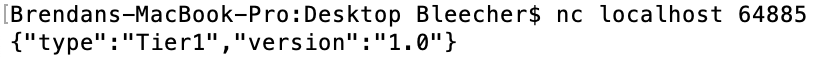
\includegraphics[width=1\textwidth]{spotifyMessage.png}
\caption{Message Received from \texttt{Spotify} TCP Port}
\label{fig:spotifyTcpResponse}
\end{figure}

\subsection{\texttt{Spotify} UNIX Domain Sockets}
\label{sec:spotifyUnix}

\begin{table}
\centering
\begin{normalsize}
\begin{tabular}{ l | l | l }
\textbf{Name} & \textbf{Found Messages?} & \textbf{Did I Fuzz?} \\ \hline
8 \texttt{socketpair} & No & No \\ \hline
2 connected to \texttt{mDNSResponder} & No & No \\ \hline
1 connected to \texttt{launchd} & No & No \\ \hline
\end{tabular}
\caption{UNIX Domain Socket Resources for \texttt{Spotify}}
\label{tab:spotifyUnixTab}
\end{normalsize}
\end{table} 

Finally, I investigated the UNIX domain sockets that \texttt{Spotify} opened, detailed in Table~\ref{tab:spotifyUnixTab}.  For each instance of \texttt{Spotify} created during testing, the \texttt{Spotify} application would have eleven UNIX domain socket endpoints open.  These were split among one instance of the \texttt{Spotify} process and two instances of the \texttt{Spotify Helper} process.  Of these eleven endpoints, eight were created using \texttt{socketpair} and shared between the various \texttt{Spotify} processes.  There was one pair within the \texttt{Spotify} process, and another pair between each \texttt{Spotify Helper} process and the \texttt{Spotify} process.  Finally, there was a pair between the two \texttt{Spotify Helper} processes.  Since no other process was given any of these endpoints, there was no way to send any messages or attempt to fuzz these endpoints.  However, there were also three UNIX domain sockets that were connected to named UNIX sockets.  One was connected to a socket owned by both \texttt{launchd} and \texttt{syslogd}.  The security of this communication will be discussed in Section~\ref{sec:launchdUnix}.  The other two were both connected to a socket owned by \texttt{mDNSResponder}.  This will be examined in Section~\ref{sec:mdnsUnix}.

\begin{table}
\centering
\begin{scriptsize}
\begin{tabular}{ l | l | l | l }
\textbf{Form of Local IPC} & \textbf{Socket Type} & \textbf{Attack Vector} & \textbf{Result} \\ \hline
Internet Domain Socket & 1 TCP Socket & Input-based & Fuzzed with no crash \\ \hline
Internet Domain Socket & 3 UDP Sockets & Input-based & Fuzzed with no crash \\ \hline
UNIX Domain Socket & 3 named connections & Input-based & Owned by others, could not fuzz \\ \hline
UNIX Domain Socket & 8 \texttt{socketpair} endpoints & Input-based & Cannot fuzz \\ \hline
\end{tabular}
\caption{Summary of my Investigation into \texttt{Spotify}}
\label{tab:spotifyData}
\end{scriptsize}
\end{table} 

\subsection{\texttt{Spotify} Conclusion}
\label{sec:spotifyConclusion}
Based on my research into \texttt{Spotify}, summarized in Table~\ref{tab:spotifyData}, I believe that this application is fairly secure against local input-based vulnerabilities.  I was unable to crash \texttt{Spotify} using any of the open UDP or TCP sockets.  Additionally, its use of UNIX domain sockets is very secure since almost all of them are created using \texttt{socketpair} and therefore cannot be directly given input by an outside process.

\section{\texttt{VS Code}}
\label{sec:code}
\texttt{VS Code} only uses two of the forms of local IPC that I studied: local TCP connections and UNIX domain sockets.  However, the biggest reason that I chose to look at \texttt{VS Code} is because it has so many named UNIX sockets.  Additionally, some of these sockets have the same name for each instance of \texttt{VS Code} while others have random suffixes each time.  This gives an interesting contrast to study.  \texttt{VS Code} is made up of the processes \texttt{Code Helper} and \texttt{Electron}.  There is always only one running process of \texttt{Electron}, but depending on the number of windows and tabs open, there may be many running instances of Code Helper.

\subsection{\texttt{VS Code} TCP}
\label{sec:codeTcp}

\begin{table}
\centering
\begin{normalsize}
\begin{tabular}{ l | l | l }
\textbf{Port} & \textbf{Found Messages?} & \textbf{Did I Fuzz?} \\ \hline
Random & No & Yes \\ \hline
Random & No & Yes \\ \hline
\end{tabular}
\caption{TCP Resources for \texttt{VS Code}}
\label{tab:vsCodeTcpTab}
\end{normalsize}
\end{table}

\texttt{VS Code} averaged two listening TCP ports, according to my survey data in Table~\ref{tab:vsCodeTcpTab}.  The ports chosen were always random, so I needed to find the port each time I started a fuzzing session.  When I originally fuzzed these ports with random data, I was always returned the message ``WebSockets request was expected.''  After doing cursory research on Google, I found that this meant that it was looking for an HTTP request.  Therefore, I created an HTTP GET request to get the repository holding the research for this thesis from GitHub and used this as my genuine communication example.

When I used this message to fuzz the \texttt{VS Code} endpoint, the program would end between fifty and one hundred messages into fuzzing because the port had been closed.  Whenever I went back to my open instance of \texttt{VS Code}, my \texttt{VIM} extension no longer worked.  \texttt{VS Code} was no longer using \texttt{VIM} keybindings nor was it using the normal keyboard keys and shortcuts.  This experiment was repeated three times, and each time the \texttt{VIM} extension crashed.  This finding represents either a bug in the way that \texttt{VS Code} or its \texttt{VIM} extension parses input to its random TCP ports since it does not correctly handle the input I was sending.  This bug could also constitute a vulnerability, which, if exploitable, could allow an attacker to either hijack execution or disclose personal information.  Therefore, this is a significant finding.

\subsection{\texttt{VS Code} UNIX Domain Sockets}
\label{sec:codeUnix}

\begin{table}
\centering
\begin{normalsize}
\begin{tabular}{ l | l | l }
\textbf{Name} & \textbf{Found Messages?} & \textbf{Did I Fuzz?} \\ \hline
20 \texttt{socketpair} & No & No \\ \hline
`main' & Yes & Yes \\ \hline
`shared' & Yes & Yes \\ \hline
`git' & No & Yes \\ \hline
`ipc' & No & Yes \\ \hline
10 connections to other processes & No & No \\ \hline
\end{tabular}
\caption{UNIX Domain Socket Resources for \texttt{VS Code}}
\label{tab:vsCodeUnixTab}
\end{normalsize}
\end{table} 

In addition to its TCP sockets, \texttt{VS Code} also has many UNIX domain sockets,  four of which are named and shown in Table~\ref{tab:vsCodeUnixTab}.  One is named based on the version number and the word `main', hereafter known as the main socket.  One is named off of the version number and the word `shared', known as the shared socket.  The last two are named using either the word `git' or `ipc' and followed by a random suffix; I call these the git and ipc sockets, respectively.  These random socket names were likely created with the \texttt{mktemp} library call or utility to create a name that is guaranteed to be unique in the filesystem.

When fuzzing the main socket, I used a six-byte message as my seed that I found was sent when the application was being closed.  However, after fuzzing over 500,000 times with variations of this message, \texttt{VS Code} did not crash or function incorrectly.

However, since the name of the main socket does not change, I deleted the socket from the filesystem and created it again myself.  Then, I tried to open \texttt{VS Code}.  I received a message saying that another instance of \texttt{VS Code} was running.  I had created a Denial-of-Service attack by opening the main socket myself.  \texttt{VS Code} must have checked the return value of the bind call, seen that this name in the filesystem was already taken, and decided that an instance was already running.  Since I had created this socket, no other instance of \texttt{VS Code} would be able to run without first deleting the socket from the file system and killing any process that had it open or restarting the entire machine.

The next socket that I looked at was the shared socket.  By impersonating this socket, I found a forty-five byte message that was sent from a client when \texttt{VS Code} started.  Using this message to fuzz the shared socket, I was unable to cause a crash after 500,000 iterations.

I then investigated the git socket.  Since it has a random suffix, I could not create this socket before I had a running instance of \texttt{VS Code}.  However, I did delete the socket and recreate it myself, but did not find any sample messages.  When I attempted to fuzz this socket, I received a BrokenPipeError in Python after two messages were successfully sent.  A BrokenPipeError in Python means that the remote communication endpoint has closed the socket for reading, but the local endpoint is still sending data.  I hypothesize, since this error always occurred after two successful sends, that this could be a security measure put in place by \texttt{VS Code}.  This socket may never expect to see more than two messages from the same client, so it closes that connection for reading after receiving two to prevent something nefarious from happening.  It is also possible that this could be an error in the way that the socket is being used, but since it always occurred after exactly two successful messages, I believe that it is for security purposes.

The last named socket is the ipc socket.  Again, this socket has a random suffix so I cannot create it before I started \texttt{VS Code}.  Once I started \texttt{VS Code}, I would see in the output of \texttt{lsof} that this socket was open and connected to another UNIX domain socket owned by another instance of the \texttt{Code Helper} process.  However, when I tried to delete this socket from the file system to create my own version, I found that this socket did not exist.  If I tried to connect to the ipc socket as a client, I would receive an error stating that the file did not exist.

This means that \texttt{VS Code} created this socket and created the connections it needed while the application was starting, then immediately called \texttt{unlink} on the socket.  This would reduce the link count of the socket, decrementing it to zero.  Since the link count was zero, it would no longer show up in the filesystem, which explains my findings.  However, since this socket was still being used, it would not actually be garbage collected by the system until all processes referencing the file exited.  Therefore, the two separate \texttt{Code Helper} processes were able to connect and still communicate while being sure that no other process could snoop on the communication.

I do not know why \texttt{VS Code} uses this system for the ipc socket, especially when it has so many \texttt{socketpair} sockets open at the same time, even between the two processes connected by the ipc socket.  However, the usage of the ipc socket is, in practice, the same as a \texttt{socketpair} socket since no other process can join the conversation.

\begin{table}
\centering
\begin{scriptsize}
\begin{tabular}{ l | l | l | l }
\textbf{Form of Local IPC} & \textbf{Socket Type} & \textbf{Attack Vector} & \textbf{Result} \\ \hline
Internet Domain Socket & 2 TCP Sockets & Input-based & Fuzzing caused VIM extension to crash \\ \hline
UNIX Domain Socket & Named ``main'' socket & Input-based & Fuzzed with no crash \\ \hline
UNIX Domain Socket & Named ``main'' socket & Server impersonation & Denial-of-Service Attack \\ \hline
UNIX Domain Socket & Named ``git'' socket & Input-based & Possible security feature \\ \hline
UNIX Domain Socket & Named ``ipc'' socket & Input-based & Cannot fuzz \\ \hline
UNIX Domain Socket & Named ``shared'' socket & Input-based & Fuzzed with no crash \\ \hline
UNIX Domain Socket & 18 \texttt{socketpair} endpoints & Input-based & Cannot fuzz \\ \hline
\end{tabular}
\caption{Summary of my Investigation into \texttt{VS Code}}
\label{tab:codeData}
\end{scriptsize}
\end{table} 

\subsection{\texttt{VS Code} Conclusion}
\label{sec:codeConclusion}
My research, outlined in Table~\ref{tab:codeData}, has shown that \texttt{VS Code} is not immune to input-based vulnerabilities over local IPC.  Through my fuzzing, I crashed a \texttt{VIM} extension that was open in \texttt{VS Code}.  Additionally, I caused a Denial-of-Service attack by opening the main UNIX socket before opening the \texttt{VS Code} application.  While \texttt{VS Code} does use some security features, like closing the connection once the git socket receives two messages and immediately \texttt{unlink}ing the ipc socket, it still is vulnerable and must be fixed, lest it be found exploitable.

\section{\texttt{launchd}}
\label{sec:launchd}
I chose to test \texttt{launchd} because it is the process that helps boot the machine, as well as starting many services, or daemons.  It is responsible for creating and maintaining many necessary services, such as networking, logging and showing images on the screen.  \texttt{launchd} uses local TCP and UDP sockets, as well as many named UNIX domain sockets.

\subsection{\texttt{launchd} TCP}
\label{sec:launchdTcp}

\begin{table}
\centering
\begin{normalsize}
\begin{tabular}{ l | l | l }
\textbf{Port} & \textbf{Found Messages?} & \textbf{Did I Fuzz?} \\ \hline
Could not replicate & No & No \\ \hline
\end{tabular}
\caption{TCP Resources for \texttt{launchd}}
\label{tab:launchdTcpTab}
\end{normalsize}
\end{table} 

My survey results showed that \texttt{launchd} averaged four open TCP sockets at a time, seen in Table~\ref{tab:launchdTcpTab}.  However, no matter when I tried to find these sockets on my own computer, I was unable to find an open TCP socket that \texttt{launchd} was listening on.  Therefore, since I could not recreate this result, I was unable to fuzz any TCP sockets for \texttt{launchd}.

\subsection{\texttt{launchd} UDP}
\label{sec:launchdUdp}

\begin{table}
\centering
\begin{normalsize}
\begin{tabular}{ l | l | l }
\textbf{Port} & \textbf{Found Messages?} & \textbf{Did I Fuzz?} \\ \hline
137 & Yes & Yes \\ \hline
138 & Yes & Yes \\ \hline
\end{tabular}
\caption{UDP Resources for \texttt{launchd}}
\label{tab:launchdUdpTab}
\end{normalsize}
\end{table} 

\texttt{launchd} averaged two open UDP sockets, as shown in Table~\ref{tab:launchdUdpTab}, one listening on port 137 and the other on port 138, both listening on any interface.  These ports are the netbios-ns and netbios-dgm ports.  NetBIOS was a way for computers to communicate on a local network.  The netbios-ns port was used to get the NetBIOS name of another computer on the network and netbios-dgm was used to send datagrams within the network.  I used \textit{Wireshark} to find sample messages being sent to these ports, and found two examples of mDNS responses.  To fuzz these sockets, my program randomly chooses one message, sends it to \textit{radamsa} to modify and then randomly chooses a port to send it to.  In this way, both messages were randomly being sent to both ports, maximizing the possiblity of a crash.  Even with this process, fuzzing both of these ports did not cause \texttt{launchd} to crash.

\subsection{\texttt{launchd} UNIX Domain Sockets}
\label{sec:launchdUnix}

\begin{table}
\centering
\begin{normalsize}
\begin{tabular}{ l | l | l }
\textbf{Name} & \textbf{Found Messages?} & \textbf{Did I Fuzz?} \\ \hline
/private//var/run/syslog & No & Yes \\ \hline
/var/rpc/ncalrpc/NETLOGON & No & Yes \\ \hline
/var/run/vpncontrol.sock & No & Yes \\ \hline
/var/run/systemkeychaincheck.socket & No & Yes \\ \hline
/var/run/portmap.socket & No & Yes \\ \hline
/var/run/usbmuxd & No & Yes \\ \hline
30 other named sockets & No & No \\ \hline
\end{tabular}
\caption{UNIX Domain Socket Resources for \texttt{launchd}}
\label{tab:launchdUnixTab}
\end{normalsize}
\end{table} 

Unlike many other processes, a majority of \texttt{launchd}'s UNIX domain sockets were not \texttt{socketpair} sockets, indicated in Table~\ref{tab:launchdUnixTab}.  In fact, \texttt{launchd} only had named UNIX domain sockets and had no \texttt{socketpair} endpoints.  While the survey results show that \texttt{launchd} had on average thirty-six open UNIX domain sockets, each socket was opened twice, so there were only eighteen different sockets open.  I attempted to fuzz six of these, representing one-third of the open sockets.  I was unable to find sample messages for any of these UNIX domain sockets, so I used the same sample messages from fuzzing the \texttt{launchd} UDP sockets as the seeds for my UNIX domain socket messages.

Every running application that does logging connects to a named socket owned by \texttt{launchd}, so this was the first socket that I fuzzed.  \texttt{Spotify}, \texttt{VS Code} and \texttt{mDNSResponder} all had a connection to this socket.  This socket was a datagram UNIX socket, and the only one that I found in my research.  I fuzzed this socket over 500,000 times and was not able to crash \texttt{launchd}.  I had the same result with two stream sockets that worked with remote procedure calls and a VPN.

The other three UNIX sockets that I attempted to fuzz were part of the system keychain, a port-mapping software, and the software that multiplexes access to the USB port.  While fuzzing these sockets, a BrokenPipeError would be thrown often, and quite regularly.  The system keychain socket would throw the error after one or two messages were sent successfully, then to every message for a short time period after.  Similarly, when fuzzing the port-mapping socket, the error would occur after about forty messages, and then to every message from every connection for a short time.  This seems to show that the process owning these sockets sees that too many messages were being sent, and could be malicious.  It then closes the socket for reading for a short amount of time to hopefully discourage the malicious user from continuing.

The USB socket also would throw a BrokenPipeError after the first message it received from every single connection.  Like with the git UNIX domain socket from \texttt{VS Code} in Section~\ref{sec:codeUnix}, this could be a security feature.  Also like \texttt{VS Code}, it is difficult to tell the exact motivation behind this function, or even if it is intended.  However, based on my research, it is plausible that this error is meant to decrease the likelihood of an input-based attack.

\begin{table}
\centering
\begin{scriptsize}
\begin{tabular}{ l | l | l | l }
\textbf{Form of Local IPC} & \textbf{Socket Type} & \textbf{Attack Vector} & \textbf{Result} \\ \hline
Internet Domain Socket & 4 TCP Sockets & Input-based & Could not reproduce \\ \hline
Internet Domain Socket & 2 UDP Sockets & Input-based & Fuzzed with no crash \\ \hline
UNIX Domain Socket & 3 named sockets & Input-based & Fuzzed with no crash \\ \hline
UNIX Domain Socket & 3 named sockets & Input-based & Possible security feature \\ \hline
\end{tabular}
\caption{Summary of my Investigation into \texttt{launchd}}
\label{tab:launchdData}
\end{scriptsize}
\end{table} 

\subsection{\texttt{launchd} Conclusion}
\label{sec:launchdConclusion}
From my research, shown in Table~\ref{tab:launchdData}, \texttt{launchd} seems to be secure against many local IPC-based input attacks.  I could not recreate its TCP sockets and fuzzing its UDP sockets never caused a crash.  While it has many named UNIX domain sockets, it appears that many of these implement some sort of security plan to diminish the possibility of input-based attacks.  The sockets that do not seem to have this plan did not cause a crash of \texttt{launchd} while being fuzzed, so they are secure as far as I have tested.

\section{\texttt{mDNSResponder}}
\label{sec:mdns}
The final process that I tested is \texttt{mDNSResponder}, which is responsible for different parts of networking, including some aspects of DNS, AirDrop, and finding nearby printers.  \texttt{mDNSResponder} had the largest local IPC footprint of the four applications that I studied, averaging sixty-two listening UDP sockets and forty-four UNIX domain sockets.  This set up a large testing ground for my research.

\subsection{\texttt{mDNSResponder} TCP}
\label{sec:mdnsTcp}

\begin{table}
\centering
\begin{normalsize}
\begin{tabular}{ l | l | l }
\textbf{Port} & \textbf{Found Messages?} & \textbf{Did I Fuzz?} \\ \hline
Random & No & No \\ \hline
\end{tabular}
\caption{TCP Resources for \texttt{mDNSResponder}}
\label{tab:mdnsTcpTab}
\end{normalsize}
\end{table} 

According to my survey, \texttt{mDNSResponder} had, on average, one TCP socket listening on any interface, seen in Table~\ref{tab:mdnsTcpTab}.  However, this socket was always in the `CLOSED' state, which means that it has not started to listen yet, or had a connection and closed it and is not yet listening for any more.  Therefore, since this socket was not listening for incoming connections, I could not fuzz the single, local \texttt{mDNSResponder} TCP socket.

\subsection{\texttt{mDNSResponder} UDP}
\label{sec:mdnsUdp}

\begin{table}
\centering
\begin{normalsize}
\begin{tabular}{ l | l | l }
\textbf{Port} & \textbf{Found Messages?} & \textbf{Did I Fuzz?} \\ \hline
5353 & Yes & Yes \\ \hline
5353 & Yes & Yes \\ \hline
62 Random Ports & No & Yes, Fuzzed 6 \\ \hline
\end{tabular}
\caption{UDP Resources for \texttt{mDNSResponder}}
\label{tab:mdnsUdpTab}
\end{normalsize}
\end{table} 

\texttt{mDNSResponder} always has two sockets listening on the mdns port, port number 5353, shown in Table~\ref{tab:mdnsUdpTab}.  This can be done by setting the SO\_REUSEPORT flag on all of the sockets before binding, and can help load-balance across multiple sockets.  I found two sample messages sent to port 5353 by using \textit{Wireshark}, and used these as my seed messages for fuzzing.  Each iteration, one of the two messages was randomly selected and then randomly modified, then sent to the port.  I was unable to cause a crash of \texttt{mDNSResponder} nor could I sense a slowdown in Internet speed from this fuzzing.

I then looked at the other, random UDP ports that mDNSResponder had open.  I could not find any messages for any of these ports, so I used the messages I found for port 5353 to fuzz these ports.  Since these ports were all random, I randomly chose six to fuzz.  I was unable to crash mDNSResponder nor feel a distinct difference in Internet speed.

\subsection{\texttt{mDNSResponder} UNIX Domain Sockets}
\label{sec:mdnsUnix}

\begin{table}
\centering
\begin{normalsize}
\begin{tabular}{ l | l | l }
\textbf{Name} & \textbf{Found Messages?} & \textbf{Did I Fuzz?} \\ \hline
4 \texttt{socketpair} & No & No \\ \hline
/var/run/mDNSResponder & Yes & Yes \\ \hline
\end{tabular}
\caption{UNIX Domain Socket Resources for \texttt{mDNSResponder}}
\label{tab:mdnsUnixTab}
\end{normalsize}
\end{table} 

As mentioned before and described in Table~\ref{tab:mdnsUnixTab}, \texttt{mDNSResponder} has over forty UNIX domain sockets open at any one time.  There are four \texttt{socketpair} endpoints open within the process, representing four of the total UNIX socket endpoints.  The other forty are all connected to the same named UNIX domain socket.  I fuzzed this named socket using a thirty-two-byte message that I received when I created my own version of this socket.  Even after 500,000 iterations, Internet traffic was not noticably slower and \texttt{mDNSResponder} had not crashed.

However, when I created my own instance of the named UNIX socket after deleting the real version, most Internet traffic from my computer failed.  All webpages failed to load, and I could no longer get music from \texttt{Spotify}.  This was essentially a Denial-of-Service attack, where I denied access to most of the rest of the Internet.  The only way to bring back Internet access was to restart the entire machine and let \texttt{mDNSResponder} create the real socket again.

\begin{table}
\centering
\begin{scriptsize}
\begin{tabular}{ l | l | l | l }
\textbf{Form of Local IPC} & \textbf{Socket Type} & \textbf{Attack Vector} & \textbf{Result} \\ \hline
Internet Domain Socket & 1 TCP Socket & Input-based & Always CLOSED \\ \hline
Internet Domain Socket & 62 UDP Sockets & Input-based & Fuzzed with no crash \\ \hline
UNIX Domain Socket & 1 named socket & Input-based & Fuzzed with no crash \\ \hline
UNIX Domain Socket & 1 named socket & Server impersonation & Denial-of-Service Attack \\ \hline
UNIX Domain Socket & 4 \texttt{socketpair} endpoints & Input-based & Cannot fuzz \\ \hline
\end{tabular}
\caption{Summary of my Investigation into \texttt{mDNSResponder}}
\label{tab:mdnsData}
\end{scriptsize}
\end{table} 

\subsection{\texttt{mDNSResponder} Conclusion}
\label{sec:mdnsConclusion}
Based on all of my research, condensed into Table~\ref{tab:mdnsData}, it seems that \texttt{mDNSResponder} is secure against local input-based vulnerabilities.  However, if its named UNIX domain socket is deleted, the machine loses most access to the rest of the outside world.  While this attack is not an input-based attack, it uses local IPC channels as the attack vector to significantly reduce Internet access.

\chapter{Future Work}
\label{sec:futureWork}
There are many different directions that researchers could follow to build off of this work.  First, when I was fuzzing, I only consistently tested after each input if the total application crashed.  However, the one bug that I did find, crashing the VIM extension in VS Code, was only found by using the application while I was fuzzing it.  I did attempt to use each application while I fuzzed it---playing music from Spotify, writing code in VS Code, and using the Internet while fuzzing mDNSResponder---but I did not do this in an organized and reproducible fashion, nor did I do it the entire duration of fuzzing.

I would also like to look at how these applications work by tracing them as well.  I was unable to acquire a computer that I had \texttt{sudo} access to that I felt comfortable turning off System Integrity Protections, so I was unable to trace any application.  By tracing an application, I would be able to see the exact system calls and arguments used for each system call, and get a better understanding of exactly what each application was doing.  This could let me have a more targeted approach to my fuzzing.

Finally, I want to look deeper into the BrokenPipeErrors that I received when fuzzing VS Code and launchd.  I hypothesize that these errors are evidence of security features that help prevent against fuzzing and attempts to find input-based vulnerabilities.

\chapter{Discussion}
\label{sec:discussion}
In the course of my research, I have found ways for developers to create secure software, as well as practices that can produce security problems.  By looking at these four applications---\texttt{Spotify}, \texttt{VS Code}, \texttt{launchd}, and \texttt{mDNSResponder}---I identified three possible attacks.  First, there is a bug in either the \texttt{VIM} extension of \texttt{VS Code} or \texttt{VS Code} itelf when parsing incoming TCP data.  I was able to crash the \texttt{VIM} extension by fuzzing this socket with a bogus HTTP GET request.  This bug could be a vulnerability that could be exploitable.

I also found two Denial-of-Service attacks, one each against \texttt{VS Code} and \texttt{mDNSResponder}.  In \texttt{VS Code}, I could create the main UNIX domain socket before running the application, and therefore the actual \texttt{VS Code} instance would not start.  For \texttt{mDNSResponder}, I removed its named UNIX domain socket and remade it myself, which essentially made applications that need Internet access unusable.  These last two vulnerabilities are similar to those found by Bui et. al. in their Man-in-the-Machine paper, which found client or server impersonation attacks in many different applications~\cite{MitMa}.

I expanded their research by also looking at UNIX domain sockets and found interesting security holes, described above, as well as ways that these can contribute to secure systems.  As noted before, \texttt{socketpair} UNIX domain sockets are more secure than the other forms of local IPC that I investigated because it is impossible to join them from an outside process.  A process must be explicitly given access to send or receive data over one of the sockets, creating much stricter access control than any other form of local IPC that I looked at.

In addition to the \texttt{socketpair} UNIX sockets, some applications improve their security by closing a socket whenever it has received the maximum number of messages that it expects.  For example, the named USB UNIX domain socket owned by \texttt{launchd} would close any connection after receiving a single message.  I believe that this was done to prevent possible fuzzing attacks and other input-based attacks.

These vulnerabilities could be solved by following a few common-sense fixes.  For example, an application should randomize the name of a named UNIX domain socket or named pipe, so that a malicious process cannot impersonate it before the application starts.  If a resource must have a predictable name, then applications must check the return value of calling \texttt{bind} to ensure that the bind has succeeded and that there is not already an instance of that named object.

Another solution is to think about the complexity of the input language that a process should accept when designing the communication protocol.  Developers need to consider if it is possible to prove that a parser accepts exactly the desired input language.  If it is not possible, then the protocol needs to be redesigned so that it can be.  This will help reduce the prevalence of input-based attacks.

Finally, software developers need to follow the same best-practices used for Internet communication for local IPC.  This includes encrypting every message and confirming the identity of the remote end of a communication channel.  This way, the security of local IPC will not be lagging behind networked IPC as it is today.

As time goes on, applications will become more secure as better practices are created and adopted.  However, as my thesis shows, time is not the only solution to creating safe and secure software.  We as developers need to think about ways to prove that our software is secure before we design it, not after.  We must never assume that we have found all of the possible bugs in our software and must continue to test continuously and rigorously.  These practices will create a safer virtual world to live in.


\appendix
\chapter{Code Samples}
\label{sec:codeSamples}
This appendix contains samples of code to use the three forms of local IPC that I studied in my thesis.  There are examples of reading from and writing to a named pipe, communicating through TCP and UDP over the loopback interface, and using stream- and datagram-based UNIX domain sockets.

\section{Writing to a Named Pipe}
\label{appendix:namedPipeWrite}
\lstinputlisting{pipeWriter.c}

\section{Reading from a Named Pipe}
\label{appendix:namedPipeRead}
\lstinputlisting{pipeReader.c}

\section{Loopback Interface TCP Server}
\label{appendix:loopbackTcpServer}
\lstinputlisting{streamLocalhostServer.c}

\section{Loopback Interface TCP Client}
\label{appendix:loopbackTcpClient}
\lstinputlisting{streamLocalhostClient.c}

\section{Loopback Interface UDP Server}
\label{appendix:loopbackUdpServer}
\lstinputlisting{datagramLocalhostServer.c}

\section{Loopback Interface UDP Client}
\label{appendix:loopbackUdpClient}
\lstinputlisting{datagramLocalhostClient.c}

\section{UNIX Domain Socket Stream Server}
\label{appendix:unixStreamServer}
\lstinputlisting{streamUnixServer.c}

\section{UNIX Domain Socket Stream Client}
\label{appendix:unixStreamClient}
\lstinputlisting{streamUnixClient.c}

\section{UNIX Domain Socket Datagram Server}
\label{appendix:unixDgramServer}
\lstinputlisting{datagramUnixServer.c}

\section{UNIX Domain Socket Datagram Client}
\label{appendix:unixDgramClient}
\lstinputlisting{datagramUnixClient.c}

\section{\texttt{socketpair} UNIX Domain Sockets}
\label{appendix:unixSocketpair}
\lstinputlisting{socketpair.c}

\chapter{Process Groups}
\label{appendix:processGroups}
Below is a list of all of the groups that I made to look at local IPC resources on the application level instead of the process level.  For each block, the first name on the left in all capital letters is the application name, and all names to the right are the processes that make up the application.

\begin{scriptsize}
\begin{longtable}[l]{ l | l | l | l }
    \hline
    SPOTIFY & Spotify & Spotify Helper & SpotifyWebHelper \\ \hline \hline
    DROPBOX & Dropbox & Dropbox Web Helper & \\ \hline \hline
    CHROME & Google Chrome & Google Chrome Helper & \\ \hline \hline
    AIRPLAY & AirPlayUIAgent & AirPlayXPCHelper & \\ \hline \hline
    SIRI & Siri & com.apple.siri-distributed-eval & \\ \hline \hline
    SAFARI & Safari & com.apple.Safari.SafeBrowsing.S & com.apple.Safari.SandboxBroker \\ \hline
    & com.apple.Safari.SearchHelper & SafariCloudHistoryPushAgent & com.apple.WebKit.Networking \\ \hline
    & com.apple.WebKit.WebContent & & \\ \hline \hline
    R & R & RStudio & \\ \hline \hline
    EXCEL & Microsoft Excel & & \\ \hline \hline
    POWERPOINT & Microsoft PowerPoint & & \\ \hline \hline
    WORD & Microsoft Word & & \\ \hline \hline
    ITUNES & iTunes & iTunesHelper & \\ \hline \hline
    SLACK & Slack & Slack Helper & \\ \hline \hline
    PYTHON & Python & python3.6 & Microsoft.Python.LanguageServer \\ \hline \hline
    OPERA & Opera & Opera Helper & \\ \hline \hline
    FIREFOX & Firefox & & \\ \hline \hline
    VS CODE & Electron & Code Helper & \\ \hline \hline
    ATOM & Atom & Atom Helper & \\ \hline \hline
    EPIC GAMES/FORTNITE & UnrealCEFSubProcess & FortniteClient-Mac-Shipping & EpicGamesLauncher-Mac-Shipping \\ \hline \hline
    AVAST & com.avast.proxy & com.avast.wifiguard & com.avast.helper \\ \hline
    & com.avast.fileshield & com.avast.service & com.avast.daemon \\ \hline \hline
    APPLE PHOTOS & com.apple.photomodel & com.apple.photomoments & \\ \hline \hline
    APPLE PREFERENCES & com.apple.preference.nerwork.re & com.apple.preference.desktopscr & com.apple.preference.displays.A \\ \hline
    & com.apple.preference.energysave & com.apple.preference.general.re & \\ \hline \hline
    CALL HISTORY & CallHistorySyncHelper & CallHistoryPluginHelper & \\ \hline \hline
    CALENDAR & Calendar & CalendarAgent & \\ \hline \hline
    PRINTING & printtool & PrintUITool & \\ \hline \hline
    MAIL & Mail & & \\ \hline \hline
    BLUETOOTH & bluetoothd & blued & bluetoothaudiod \\ \hline \hline
    ADDRESS BOOK & AddressBookSourceSync & com.apple.AddressBook.ContactsA & com.apple.AddressBook.FaceTimeS \\ \hline \hline
    CREATIVE CLOUD & Core Sync & Creative Cloud & Adobe Desktop Server \\ \hline \hline
    CORE SERVICES & coreservicesd & CoreServicesUIAgent & \\ \hline \hline
    MDS & mds & mds\_stores \\ \hline \hline
    EXPRESS VPN & ExpressVPN & expressvpnd & \\ \hline \hline
    SPOTLIGHT & Spotlight & SpotlightNetHelper & \\ \hline \hline
    CARBONITE & CarboniteStatus & CarboniteDaemon & \\ \hline \hline
    ICON SERVICES & iconservicesd & iconservicesagent & \\ \hline \hline
    RDR CEF & RdrCEF & RdrCEF Helper & \\ \hline \hline 
    SPINDUMP & spindump & spindump.agent & \\ \hline \hline



\end{longtable}
\end{scriptsize}

\chapter{Complete Data Table}
\label{appendix:allData}
Below is the complete data table that I assembled from the results of my survey.  It shows the application name, the number of machines it was running on, and the local IPC footprint of that application.  All of the columns below represent averages found from my survey.


\setlength\LTleft{-1in}
\begin{adjustwidth}{-2in}{}
\begin{scriptsize}
\begin{longtable}[l]{ l | r | r | r | r | r | r }
    \hline
    APP NAME &  MACHINES &  FIFOS &  PIPES & LOCAL TCP(TOTAL) & LOCAL UDP(TOTAL) & UNIX \\ \hline
    \endhead
    accountsd &  8 &  0 &  0 &  0 (0) &  0 (0) &  1 \\ \hline
    Acrobat Updater & 2 &  0 &  3 &  0 (0) &  0 (0) &  2 \\ \hline
    ADDRESS BOOK & 4 &  0 &  0 &  0 (2) &  0 (0) &  2 \\ \hline
    Adobe CEF Helper & 2 &  0 &  4 &  0 (0) &  0 (0) &  5 \\ \hline
    Adobe Installer & 1 &  2 &  0 &  0 (0) &  0 (0) &  0 \\ \hline
    AdobeCRDaemon &  1 &  0 &  0 &  0 (0) &  0 (0) &  1 \\ \hline
    AdobeIPCBroker & 2 &  0 &  0 &  0 (0) &  0 (0) & 10 \\ \hline
    AdobeReader &  2 &  0 &  0 &  0 (0) &  0 (0) &  7 \\ \hline
    AdobeUpdateDaemon &  2 &  2 &  0 &  0 (0) &  0 (0) &  0 \\ \hline
    AIRPLAY & 22 &  0 &  0 &  0 (1) &  2 (2) &  5 \\ \hline
    airportd &  22 &  0 &  0 &  0 (0) &  10 (10) &  3 \\ \hline
    akd & 18 &  0 &  0 &  0 (0) &  0 (0) &  1 \\ \hline
    APPLE PHOTOS & 1 &  0 &  0 &  0 (0) &  0 (0) &  4 \\ \hline
    APPLE PREFERENCES &  1 &  0 &  0 &  0 (0) &  3 (3) &  5 \\ \hline
    appleeventsd & 1 &  0 &  0 &  0 (0) &  0 (0) &  1 \\ \hline
    AppleIDAuthAgent & 1 &  0 &  0 &  0 (0) &  0 (0) &  2 \\ \hline
    AppleMobileDeviceHelper &  8 &  0 &  2 &  0 (0) &  0 (0) &  3 \\ \hline
    AppleSpell & 1 &  0 &  226 &  0 (0) &  0 (0) &  1 \\ \hline
    AppStats & 1 &  0 &  2 &  0 (0) &  0 (0) &  2 \\ \hline
    appstoreagent & 14 &  0 &  0 &  0 (0) &  0 (0) &  1 \\ \hline
    AppTech &  2 &  0 &  3 &  0 (0) &  0 (0) &  2 \\ \hline
    apsd &  22 &  0 &  0 &  0 (2) &  0 (0) &  4 \\ \hline
    ARDAgent & 1 &  0 &  0 &  1 (1) &  2 (2) &  1 \\ \hline
    askpermissiond & 1 &  0 &  0 &  0 (0) &  0 (0) &  1 \\ \hline
    AssetCacheLocatorService & 3 &  0 &  0 &  0 (0) &  0 (0) &  2 \\ \hline
    assistantd &  13 &  0 &  0 &  0 (1) &  1 (1) &  0 \\ \hline
    ath &  3 &  0 &  2 &  0 (0) &  0 (0) &  5 \\ \hline
    ATOM & 5 &  0 & 36 &  0 (3) &  0 (0) & 10 \\ \hline
    authd &  1 &  0 &  0 &  0 (0) &  0 (0) &  1 \\ \hline
    AVAST &  1 &  0 &  8 & 2 (56) &  0 (0) & 84 \\ \hline
    avconferenced &  9 &  0 &  0 &  1 (1) &  4 (4) &  1 \\ \hline
    awdd & 1 &  0 &  0 &  0 (0) &  0 (0) &  1 \\ \hline
    backgroundtaskmanagementagent & 19 &  0 &  0 &  0 (0) &  0 (0) &  1 \\ \hline
    Backup and Sync &  1 &  0 &  7 & 0 (15) &  0 (0) &  2 \\ \hline
    bash &  22 &  0 &  1 &  0 (0) &  0 (0) &  1 \\ \hline
    biometrickitd &  2 &  0 &  0 &  0 (1) &  0 (0) &  1 \\ \hline
    bird & 5 &  0 &  0 &  0 (0) &  0 (0) &  1 \\ \hline
    BlueJeans &  1 &  0 &  6 &  1 (1) &  0 (0) &  0 \\ \hline
    BLUETOOTH & 19 &  0 &  0 &  0 (0) &  3 (3) &  5 \\ \hline
    Calculator & 1 &  0 &  0 &  0 (0) &  0 (0) &  1 \\ \hline
    CALENDAR &  13 &  0 &  0 &  0 (2) &  0 (0) &  2 \\ \hline
    CALLHISTORY &  1 &  0 &  0 &  0 (0) &  0 (0) &  2 \\ \hline
    callservicesd &  2 &  0 &  0 &  0 (0) &  0 (0) &  1 \\ \hline
    CalNCService & 1 &  0 &  0 &  0 (0) &  0 (0) &  1 \\ \hline
    captiveagent &  15 &  0 &  0 &  0 (0) &  0 (0) &  2 \\ \hline
    CARBONITE &  1 &  0 & 34 &  2 (5) &  0 (0) &  4 \\ \hline
    cfbackd &  1 &  0 &  0 &  0 (0) &  0 (0) &  5 \\ \hline
    cfprefsd & 5 &  0 &  0 &  0 (0) &  0 (0) &  1 \\ \hline
    CHROME &  16 &  0 & 50 & 1 (26) &  1 (8) & 38 \\ \hline
    CiscoVideoGuardMonitor & 1 &  0 &  8 &  2 (2) &  0 (0) &  0 \\ \hline
    cloudd &  19 &  0 &  0 &  0 (2) &  0 (0) &  1 \\ \hline
    cloudfamilyrestrictionsd & 1 &  0 &  0 &  0 (0) &  0 (0) &  1 \\ \hline
    cloudpaird & 1 &  0 &  0 &  0 (0) &  0 (0) &  1 \\ \hline
    cloudphotosd & 1 &  0 &  0 &  0 (0) &  0 (0) &  3 \\ \hline
    CMFSyncAgent & 1 &  0 &  0 &  0 (0) &  0 (0) &  1 \\ \hline
    com.apple.AmbientDisplayAgent &  4 &  0 &  0 &  0 (0) &  0 (0) &  1 \\ \hline
    com.apple.appkit.xpc.openAndSav & 20 &  0 &  0 &  0 (0) &  0 (0) &  1 \\ \hline
    com.apple.BKAgentService & 4 &  0 &  0 &  0 (0) &  0 (0) &  1 \\ \hline
    com.apple.CommerceKit.Transacti &  3 &  0 &  0 &  0 (3) &  0 (0) &  2 \\ \hline
    com.apple.dock.extra & 1 &  0 &  0 &  0 (0) &  0 (0) &  1 \\ \hline
    com.apple.geod & 7 &  0 &  0 &  0 (2) &  0 (0) &  3 \\ \hline
    com.apple.hiservices-xpcservice &  1 &  0 &  0 &  0 (0) &  0 (0) &  1 \\ \hline
    com.apple.iCloudHelper & 2 &  0 &  0 &  0 (1) &  0 (0) &  1 \\ \hline
    com.apple.MediaLibraryService &  3 &  0 &  0 &  0 (0) &  0 (0) &  1 \\ \hline
    com.apple.PerformanceAnalysis.a &  3 &  0 &  0 &  0 (0) &  0 (0) &  1 \\ \hline
    com.apple.security.pboxd &  17 &  0 &  0 &  0 (0) &  0 (0) &  1 \\ \hline
    com.apple.speech.speechsynthesi &  1 &  0 &  0 &  0 (0) &  0 (0) &  1 \\ \hline
    com.apple.tonelibraryd & 1 &  0 &  0 &  0 (0) &  0 (0) &  1 \\ \hline
    com.symantec.SymLUHelper & 2 &  0 &  0 &  0 (0) &  0 (0) &  2 \\ \hline
    CommCenter &  20 &  0 &  0 &  0 (0) &  0 (0) &  1 \\ \hline
    commerce &  10 &  0 &  0 &  0 (2) &  0 (0) &  1 \\ \hline
    configd & 22 &  0 &  0 &  0 (0) &  4 (4) &  3 \\ \hline
    Contacts & 1 &  0 &  0 &  0 (0) &  0 (0) &  1 \\ \hline
    ContainerMetadataExtractor &  10 &  0 &  0 &  0 (0) &  0 (0) &  1 \\ \hline
    ControlStrip & 1 &  0 &  0 &  0 (0) &  0 (0) &  1 \\ \hline
    CORE SERVICES &  2 &  0 &  0 &  0 (0) &  0 (0) &  2 \\ \hline
    coreaudiod & 1 &  0 &  0 &  0 (0) &  0 (0) &  1 \\ \hline
    coreduetd &  1 &  0 &  0 &  0 (0) &  0 (0) &  1 \\ \hline
    corespeechd & 15 &  0 &  0 &  0 (0) &  0 (0) &  1 \\ \hline
    CrashReporterSupportHelper &  17 &  0 &  0 &  0 (0) &  0 (0) &  1 \\ \hline
    CREATIVE CLOUD & 2 &  2 & 19 & 2 (13) &  0 (0) & 22 \\ \hline
    cupsd & 11 &  0 &  4 &  2 (2) &  0 (0) &  2 \\ \hline
    DashboardClient &  2 &  0 &  0 &  0 (0) &  0 (0) &  1 \\ \hline
    DashlanePluginMASService & 1 &  0 &  4 &  1 (1) &  0 (0) &  0 \\ \hline
    DataDetectorsDynamicData & 1 &  0 &  0 &  0 (0) &  0 (0) &  1 \\ \hline
    dbfseventsd &  6 &  0 &  9 &  0 (0) &  0 (0) &  2 \\ \hline
    digest-service & 1 &  0 &  0 &  0 (0) &  0 (0) &  1 \\ \hline
    diskarbitrationd & 1 &  0 &  0 &  0 (0) &  0 (0) &  1 \\ \hline
    displaypolicyd &  19 &  0 &  0 &  0 (0) &  0 (0) &  1 \\ \hline
    distnoted &  1 &  0 &  0 &  0 (0) &  0 (0) &  1 \\ \hline
    Dock &  22 &  0 &  0 &  0 (0) &  0 (0) &  1 \\ \hline
    DocumentPopoverViewService & 3 &  0 &  0 &  0 (0) &  0 (0) &  1 \\ \hline
    DrCleaner &  1 &  0 &  0 &  0 (0) &  1 (1) &  2 \\ \hline
    DROPBOX &  6 &  0 & 25 & 0 (11) &  1 (1) & 68 \\ \hline
    dsAccessService &  4 &  0 &  6 &  0 (0) &  0 (0) &  0 \\ \hline
    eapolclient & 21 &  0 &  0 &  0 (0) &  1 (1) &  2 \\ \hline
    EEventManager &  1 &  0 &  0 &  1 (1) &  1 (1) &  0 \\ \hline
    EmojiFunctionRowIM\_Extension & 1 &  0 &  0 &  0 (0) &  0 (0) &  1 \\ \hline
    eoshostd & 2 &  0 &  0 &  0 (1) &  0 (0) &  0 \\ \hline
    EPIC GAMES/FORTNITE &  1 &  0 & 50 &  0 (3) &  4 (4) &  6 \\ \hline
    EpsonLowInkReminderAgent & 1 &  0 &  0 &  0 (0) &  0 (0) &  1 \\ \hline
    EXCEL &  9 &  0 &  0 &  0 (2) &  0 (0) &  3 \\ \hline
    EXPRESS VPN &  2 &  0 &  2 &  1 (1) &  1 (2) &  1 \\ \hline
    FaceTime & 1 &  0 &  0 &  0 (0) &  0 (0) &  1 \\ \hline
    familycircled & 15 &  0 &  0 &  0 (0) &  0 (0) &  1 \\ \hline
    filecoordinationd &  8 &  0 &  0 &  0 (0) &  0 (0) &  1 \\ \hline
    Finder &  22 &  0 &  0 &  0 (0) &  1 (1) &  1 \\ \hline
    findmydeviced & 20 &  0 &  0 &  0 (0) &  0 (0) &  1 \\ \hline
    FIREFOX &  1 &  0 &  9 & 0 (19) &  0 (0) & 54 \\ \hline
    Flux & 2 &  0 &  0 &  0 (0) &  0 (0) &  1 \\ \hline
    fmfd & 4 &  0 &  0 &  0 (1) &  0 (0) &  3 \\ \hline
    fontd &  1 &  0 &  0 &  0 (0) &  0 (0) &  1 \\ \hline
    FrontendAgent &  2 &  0 &  0 &  0 (0) &  0 (0) &  1 \\ \hline
    fud &  4 &  0 &  0 &  0 (0) &  0 (0) &  1 \\ \hline
    gamed &  4 &  0 &  0 &  0 (0) &  0 (0) &  1 \\ \hline
    hidd & 2 &  0 &  0 &  0 (0) &  0 (0) &  1 \\ \hline
    homed & 12 &  0 &  0 &  0 (0) &  0 (0) &  3 \\ \hline
    HP Device Monitor &  3 &  0 &  0 &  3 (3) &  0 (0) & 14 \\ \hline
    icdd &  22 &  0 &  0 &  0 (0) &  0 (0) & 10 \\ \hline
    ICON SERVICES &  1 &  0 &  0 &  0 (0) &  0 (0) &  2 \\ \hline
    identityservicesd & 22 &  0 &  0 &  0 (4) &  1 (1) &  8 \\ \hline
    IDSKeychainSyncingProxy &  1 &  0 &  0 &  0 (0) &  0 (0) &  1 \\ \hline
    Image Capture Extension &  1 &  0 &  0 &  0 (0) &  0 (0) & 11 \\ \hline
    imagent &  3 &  0 &  0 &  0 (0) &  0 (0) &  1 \\ \hline
    IMDPersistenceAgent &  1 &  0 &  0 &  0 (0) &  0 (0) &  1 \\ \hline
    IMLoggingAgent & 1 &  0 &  0 &  0 (0) &  0 (0) &  1 \\ \hline
    IMRemoteURLConnectionAgent & 7 &  0 &  0 &  0 (3) &  0 (0) &  2 \\ \hline
    IMTransferAgent &  2 &  0 &  0 &  0 (6) &  0 (0) &  0 \\ \hline
    ITUNES &  11 &  0 &  2 &  0 (4) &  0 (0) & 10 \\ \hline
    java & 2 &  0 &  0 &  1 (1) &  0 (0) &  5 \\ \hline
    Java Updater &  1 &  0 &  0 &  0 (0) &  0 (0) &  2 \\ \hline
    JavaAppLauncher &  2 &  0 &  0 &  0 (1) &  0 (0) &  3 \\ \hline
    kdc &  2 &  0 &  0 &  2 (2) &  2 (2) &  1 \\ \hline
    KernelEventAgent &  22 &  0 &  0 &  0 (0) &  0 (0) &  2 \\ \hline
    kextfind & 1 &  0 &  1 &  0 (0) &  0 (0) &  0 \\ \hline
    keyboardservicesd &  2 &  0 &  0 &  0 (0) &  0 (0) &  1 \\ \hline
    knowledge-agent &  3 &  0 &  0 &  0 (0) &  0 (0) &  1 \\ \hline
    launchd & 22 &  0 &  0 &  4 (4) &  2 (2) & 36 \\ \hline
    launchservicesd &  1 &  0 &  0 &  0 (0) &  0 (0) &  1 \\ \hline
    locationd & 22 &  0 &  4 &  0 (0) &  1 (1) &  3 \\ \hline
    LocationMenu &  11 &  0 &  0 &  0 (0) &  0 (0) &  1 \\ \hline
    logd &  19 &  0 &  0 &  0 (0) &  0 (0) &  1 \\ \hline
    loginwindow & 22 &  0 &  0 &  0 (0) &  1 (1) &  1 \\ \hline
    LookupViewService &  3 &  0 &  0 &  0 (4) &  0 (0) &  2 \\ \hline
    lsd &  1 &  0 &  0 &  0 (0) &  0 (0) &  1 \\ \hline
    lsof &  22 &  0 &  3 &  0 (0) &  0 (0) &  0 \\ \hline
    Magnet & 1 &  0 &  0 &  0 (0) &  0 (0) &  1 \\ \hline
    MAIL & 8 &  0 &  0 &  0 (4) &  0 (0) &  2 \\ \hline
    mapspushd &  3 &  0 &  0 &  0 (0) &  0 (0) &  2 \\ \hline
    mDNSResponder & 22 &  0 &  0 &  1 (3) &  62 (62) & 44 \\ \hline
    MDS & 20 &  0 &  0 &  0 (0) &  0 (0) &  2 \\ \hline
    mdwrite &  1 &  0 &  0 &  0 (0) &  0 (0) &  1 \\ \hline
    mediaremoted &  10 &  0 &  0 &  0 (0) &  0 (0) &  1 \\ \hline
    Messages &  16 &  0 &  0 &  0 (0) &  0 (0) &  1 \\ \hline
    Microsoft AutoUpdate &  1 &  0 &  0 &  0 (0) &  0 (0) &  1 \\ \hline
    Microsoft Outlook & 1 &  0 &  0 &  0 (0) &  0 (0) &  4 \\ \hline
    MirrorDisplays & 1 &  0 &  0 &  0 (0) &  0 (0) &  1 \\ \hline
    MobileDeviceUpdater & 11 &  0 &  0 &  0 (0) &  0 (0) &  3 \\ \hline
    mtmfs &  2 &  0 &  0 &  3 (3) &  0 (0) &  1 \\ \hline
    mysqld & 1 &  0 &  0 &  1 (1) &  0 (0) &  1 \\ \hline
    nehelper & 1 &  0 &  0 &  0 (0) &  0 (0) &  1 \\ \hline
    nesessionmanager & 1 &  0 &  0 &  0 (0) &  0 (0) &  3 \\ \hline
    NetAuthSysAgent &  1 &  0 &  0 &  0 (0) &  0 (0) &  1 \\ \hline
    netbiosd &  22 &  0 &  0 &  0 (0) &  2 (2) &  2 \\ \hline
    netsession\_mac & 1 &  0 &  0 &  1 (1) &  2 (2) &  1 \\ \hline
    networkd & 1 &  0 &  0 &  0 (0) &  1 (1) &  1 \\ \hline
    networkserviceproxy & 21 &  0 &  0 &  0 (0) &  0 (0) &  1 \\ \hline
    nfcd & 2 &  0 &  0 &  0 (0) &  0 (0) &  1 \\ \hline
    node & 2 &  0 &  6 &  2 (2) &  0 (0) &  4 \\ \hline
    Norton & 2 &  0 &  0 &  0 (0) &  0 (0) &  2 \\ \hline
    Notes & 10 &  0 &  0 &  0 (2) &  0 (0) &  1 \\ \hline
    NotificationCenter &  20 &  0 &  0 &  0 (0) &  0 (0) &  1 \\ \hline
    nsurlsessiond & 22 &  0 & 11 & 0 (10) &  0 (0) &  2 \\ \hline
    nsurlstoraged & 20 &  0 &  0 &  0 (0) &  0 (0) &  1 \\ \hline
    ntpd & 3 &  0 &  1 &  0 (0) &  1 (8) &  1 \\ \hline
    ocspd &  1 &  0 &  0 &  0 (0) &  0 (0) &  2 \\ \hline
    Office365ServiceV2 & 4 &  0 &  0 &  1 (1) &  0 (0) &  2 \\ \hline
    OneDrive & 1 &  0 &  0 &  0 (6) &  0 (0) &  4 \\ \hline
    opendirectoryd & 1 &  0 &  0 &  0 (0) &  0 (0) &  1 \\ \hline
    OPERA &  2 &  0 & 41 & 0 (14) &  0 (5) & 27 \\ \hline
    OSDUIHelper & 15 &  0 &  0 &  0 (0) &  0 (0) &  1 \\ \hline
    p &  1 &  0 &  2 &  0 (2) &  0 (0) &  2 \\ \hline
    P72E3GC48.com.dashlane.Dashlane &  1 &  0 & 10 &  1 (1) &  0 (0) &  0 \\ \hline
    Pages &  2 &  0 &  0 &  0 (0) &  0 (0) &  2 \\ \hline
    parentalcontrolsd &  2 &  0 &  0 &  10 (10) &  0 (0) &  4 \\ \hline
    parsecd & 10 &  0 &  0 &  0 (0) &  0 (0) &  1 \\ \hline
    pbs &  7 &  0 &  0 &  0 (0) &  0 (0) &  1 \\ \hline
    pdftex & 1 &  0 &  3 &  0 (0) &  0 (0) &  0 \\ \hline
    PerfPowerServices & 15 &  0 &  0 &  0 (0) &  1 (1) &  0 \\ \hline
    photoanalysisd & 4 &  0 &  0 &  0 (0) &  0 (0) &  1 \\ \hline
    photolibraryd &  1 &  0 &  0 &  0 (0) &  0 (0) &  1 \\ \hline
    plugin-container & 1 &  0 & 20 &  0 (0) &  0 (0) & 42 \\ \hline
    pma &  1 &  0 &  0 &  0 (0) &  0 (0) &  1 \\ \hline
    powerd & 1 &  0 &  0 &  0 (0) &  0 (0) &  1 \\ \hline
    POWERPOINT &  11 &  0 &  0 &  0 (1) &  0 (0) &  3 \\ \hline
    Preview & 18 &  0 &  0 &  0 (0) &  0 (0) &  1 \\ \hline
    PRINTING & 8 &  0 &  0 &  0 (0) &  0 (0) &  2 \\ \hline
    ProtectedCloudKeySyncing & 2 &  0 &  0 &  0 (0) &  0 (0) &  1 \\ \hline
    PulseTray &  2 &  0 &  0 &  0 (0) &  0 (0) &  1 \\ \hline
    PYTHON & 2 &  0 & 17 &  1 (1) &  0 (0) & 16 \\ \hline
    QuickLookUIService & 2 &  0 &  0 &  0 (0) &  0 (0) &  1 \\ \hline
    R &  3 &  0 &  8 &  1 (1) &  0 (0) &  2 \\ \hline
    rapportd &  19 &  0 &  0 &  2 (2) &  1 (1) &  2 \\ \hline
    rcd &  1 &  0 &  0 &  0 (0) &  0 (0) &  1 \\ \hline
    RDR CEF &  2 &  0 & 14 &  0 (0) &  0 (0) &  5 \\ \hline
    ReceiverHelper & 1 &  0 &  0 &  0 (0) &  0 (0) &  1 \\ \hline
    recentsd & 1 &  0 &  0 &  0 (0) &  0 (0) &  1 \\ \hline
    remoting\_me2me\_host &  1 &  0 & 18 &  0 (1) &  0 (0) &  1 \\ \hline
    ReportCrash &  3 &  0 &  0 &  0 (0) &  0 (0) &  1 \\ \hline
    routined & 2 &  0 &  0 &  0 (0) &  0 (0) &  1 \\ \hline
    rpcsvchost &  11 &  0 &  0 &  0 (0) &  0 (0) &  1 \\ \hline
    rsession & 3 &  0 &  9 &  3 (3) &  0 (0) &  1 \\ \hline
    rtcreportingd & 14 &  0 &  0 &  0 (0) &  0 (0) &  1 \\ \hline
    SAFARI &  11 &  0 &  2 & 0 (19) &  0 (0) & 10 \\ \hline
    SCIM\_Extension & 3 &  0 &  0 &  0 (0) &  0 (0) &  1 \\ \hline
    ScopedBookmarkAgent &  1 &  0 &  0 &  0 (0) &  0 (0) &  1 \\ \hline
    screencaptureui &  1 &  0 &  0 &  0 (0) &  0 (0) &  1 \\ \hline
    secd &  20 &  0 &  0 &  0 (0) &  0 (0) &  1 \\ \hline
    sharedfilelistd &  1 &  0 &  0 &  0 (0) &  0 (0) &  1 \\ \hline
    sharingd &  22 &  0 &  0 &  0 (0) &  5 (5) &  6 \\ \hline
    SidecarRelay & 8 &  0 &  0 &  0 (0) &  0 (0) &  1 \\ \hline
    Similar Photo Cleaner &  1 &  0 &  0 &  0 (0) &  0 (0) &  1 \\ \hline
    SIRI & 9 &  0 &  0 &  0 (0) &  0 (0) &  2 \\ \hline
    SiriNCService &  1 &  0 &  0 &  0 (0) &  0 (0) &  1 \\ \hline
    SLACK &  1 &  0 & 40 &  0 (3) &  0 (0) &  8 \\ \hline
    soagent &  1 &  0 &  0 &  0 (0) &  0 (0) &  1 \\ \hline
    socketfilterfw & 3 &  0 &  4 &  0 (0) &  0 (0) &  2 \\ \hline
    softwareupdated &  1 &  0 &  0 &  0 (0) &  0 (0) &  2 \\ \hline
    Spark &  1 &  0 &  0 &  0 (5) &  0 (0) &  2 \\ \hline
    SPINDUMP & 4 &  0 &  0 &  0 (0) &  0 (0) &  2 \\ \hline
    SPOTIFY & 12 &  0 & 33 &  1 (9) &  3 (3) & 10 \\ \hline
    SPOTLIGHT & 20 &  0 &  0 &  0 (5) &  0 (0) &  3 \\ \hline
    ssh-agent &  2 &  0 &  9 &  0 (0) &  0 (0) &  4 \\ \hline
    Stickies & 3 &  0 &  0 &  0 (0) &  0 (0) &  1 \\ \hline
    storeaccountd &  1 &  0 &  0 &  0 (0) &  0 (0) &  2 \\ \hline
    storeassetd &  1 &  0 &  0 &  0 (2) &  0 (0) &  2 \\ \hline
    storedownloadd & 1 &  0 &  0 &  0 (0) &  0 (0) &  2 \\ \hline
    storeuid & 1 &  0 &  0 &  0 (0) &  0 (0) &  1 \\ \hline
    SubmitDiagInfo & 1 &  0 &  0 &  0 (0) &  0 (0) &  3 \\ \hline
    sudo &  22 &  0 &  3 &  0 (0) &  0 (0) &  1 \\ \hline
    suggestd & 3 &  0 &  0 &  0 (0) &  0 (0) &  1 \\ \hline
    suhelperd & 19 &  0 &  0 &  0 (0) &  0 (0) &  1 \\ \hline
    SymDaemon &  2 &  0 &  8 &  0 (1) &  1 (1) & 16 \\ \hline
    symptomsd & 22 &  0 &  0 &  0 (0) &  1 (1) &  1 \\ \hline
    syncdefaultsd &  5 &  0 &  0 &  0 (1) &  0 (0) &  2 \\ \hline
    syslogd & 22 &  0 &  0 &  0 (0) &  1 (1) &  2 \\ \hline
    syspolicyd &  15 &  0 &  0 &  0 (0) &  0 (0) &  1 \\ \hline
    System Preferences &  4 &  0 &  0 &  0 (0) &  0 (0) &  1 \\ \hline
    systemstats & 19 &  0 &  0 &  0 (0) &  2 (2) &  1 \\ \hline
    SystemUIServer &  22 &  0 &  3 &  0 (0) &  5 (5) &  1 \\ \hline
    tccd & 1 &  0 &  0 &  0 (0) &  0 (0) &  1 \\ \hline
    Terminal &  22 &  0 &  4 &  0 (0) &  0 (0) &  1 \\ \hline
    TeXShop &  2 &  0 &  1 &  0 (0) &  0 (0) &  1 \\ \hline
    TextEdit & 7 &  0 &  0 &  0 (0) &  0 (0) &  1 \\ \hline
    timed & 19 &  0 &  0 &  0 (0) &  1 (1) &  2 \\ \hline
    TouchBarServer & 1 &  0 &  0 &  0 (0) &  0 (0) &  1 \\ \hline
    trustd & 8 &  0 &  0 &  0 (0) &  0 (0) &  2 \\ \hline
    usbmuxd & 22 &  0 &  0 &  0 (1) &  0 (0) & 10 \\ \hline
    useractivityd &  1 &  0 &  0 &  0 (0) &  0 (0) &  1 \\ \hline
    UserEventAgent &  22 &  0 &  0 &  0 (0) &  1 (1) &  4 \\ \hline
    usernoted & 16 &  0 &  0 &  0 (0) &  0 (0) &  1 \\ \hline
    vpnagentd &  2 &  0 & 23 &  1 (1) &  0 (0) &  1 \\ \hline
    VS CODE & 2 &  0 & 52 & 2 (10) &  0 (0) & 22 \\ \hline
    warmd &  1 &  0 &  0 &  0 (0) &  0 (0) &  1 \\ \hline
    WDSecurityHelper & 1 &  0 &  0 &  0 (0) &  0 (0) &  1 \\ \hline
    WeatherService & 1 &  0 &  0 &  0 (0) &  0 (0) &  1 \\ \hline
    WiFiAgent & 22 &  0 &  0 &  0 (0) &  1 (1) &  1 \\ \hline
    WiFiProxy & 20 &  0 &  0 &  0 (0) &  1 (1) &  0 \\ \hline
    wifivelocityd &  3 &  0 &  0 &  0 (0) &  2 (2) &  2 \\ \hline
    WindowServer &  18 &  0 &  0 &  0 (0) &  0 (0) &  1 \\ \hline
    wirelessproxd &  1 &  0 &  0 &  0 (0) &  0 (0) &  1 \\ \hline
    WirelessRadioManagerd & 20 &  0 &  0 &  0 (0) &  1 (1) &  0 \\ \hline
    WORD &  16 &  0 &  4 &  2 (3) &  0 (0) &  4 \\ \hline
    WunderlistHelper & 1 &  0 &  0 &  0 (0) &  0 (0) &  3 \\ \hline
    xartstorageremoted & 2 &  0 &  0 &  2 (2) &  0 (0) &  0 \\ \hline
    ZoomOpener & 3 &  0 &  4 &  1 (1) &  0 (0) &  0 \\ \hline
    zotero & 1 &  0 &  4 &  2 (4) &  0 (0) &  2 \\ \hline

     
\end{longtable}
\end{scriptsize}
\end{adjustwidth}


\bibliography{thesis}

\end{document}
